%----------------------------------------------------------------------------------------
%	PACKAGES AND OTHER DOCUMENT CONFIGURATIONS
%----------------------------------------------------------------------------------------

\documentclass[fleqn,10pt]{SelfArx} % Document font size and equations flushed left

\usepackage[english]{babel} % Specify a different language here - english by default


%----------------------------------------------------------------------------------------
%	COLUMNS
%----------------------------------------------------------------------------------------

\setlength{\columnsep}{0.55cm} % Distance between the two columns of text
\setlength{\fboxrule}{0.75pt} % Width of the border around the abstract

%----------------------------------------------------------------------------------------
%	COLORS
%----------------------------------------------------------------------------------------

\definecolor{color1}{RGB}{0,0,90} % Color of the article title and sections
\definecolor{color2}{RGB}{0,20,20} % Color of the boxes behind the abstract and headings

%----------------------------------------------------------------------------------------
%	HYPERLINKS
%----------------------------------------------------------------------------------------

\usepackage{hyperref} % Required for hyperlinks
\hypersetup{hidelinks,colorlinks,breaklinks=true,urlcolor=color2,citecolor=color1,linkcolor=color1,bookmarksopen=false,pdftitle={Title},pdfauthor={Author}}

%----------------------------------------------------------------------------------------
%	ARTICLE INFORMATION
%----------------------------------------------------------------------------------------

\JournalInfo{V8.0.0  2018} % Journal information
\Archive{} % Additional notes (e.g. copyright, DOI, review/research article)

\PaperTitle{HNB White Paper\\
A Next Generation Decentralized Economic Community
\\
} % Article title

\Authors{HNB Foundation} % Authors
%\affiliation{\textsuperscript{1}\textit{Department of Biology, University of Examples, London, United Kingdom}} % Author affiliation
%\affiliation{\textsuperscript{2}\textit{Department of Chemistry, University of Examples, London, United Kingdom}} % Author affiliation
%\affiliation{*\textbf{Contact}: © HNB Foundation 2018	Email: service@HNB.eco} % Corresponding author

\Keywords{} % Keywords - if you don't want any simply remove all the text between the curly brackets
\newcommand{\keywordname}{} % Defines the keywords heading name

\renewcommand{\abstractname}{Executive Summary}

%----------------------------------------------------------------------------------------
%	ABSTRACT
%----------------------------------------------------------------------------------------

\renewcommand{\abstractname}{\heiti Executive Summary}

\Abstract{
Just like how the Internet has changed the way we communicate, Blockchain technology is changing the way we transact with each other. The technological evolution is progressing from digitization of information to digitization of assets. Blockchain is promising the world with new disruptive ideas and compelling business value propositions:
\begin{itemize}
\item{Decentralization and total transparency}
\item{Tamp-resistance and trustless in transactional data}
\item{Disintermediation in transactions to reduce costs}
\item{Democratization and sharing in community building}
\item{Institutionalization enforced by computer codes to eliminate corruption}
\end{itemize}

Blockchain technology is presenting the world with its daunting vitality and endless possibilities. The conventional centralized and intermediary-based Internet business model will be challenged and eventually disrupted by this technology. Statistics shows that by 2025 the value generated through Blockchain is expected to be \$10 trillion, 10\% of the world GDP (\$100 trillion).

Blockchain related economies have been explosively growing since the inception of Bitcoin in 2009. However, the development of Blockchain business has still not reached the level that can support the large-scaled real time transactions for goods and services. There are three reasons:

\begin{itemize}
\item{Nascent underlying technologies}
\item{Immature economic models}
\item{Weak business operations}
\end{itemize}

With ever increasing investments, the major breakthroughs in Blockchain technology have taken place in recent years. The technologies such as smart contract of Ethereum, grapheme technology of EOS, evolution of consensus mechanism from PBFT, POW to POS, DPOS as well as a variety of hybrid mechanisms, Lightning Network and zero-knowledge proofs, have greatly improved security, scalability and TPS in Blockchain applications, which laid a solid foundation for the evolution of the next generation of Blockchain applications.

HNB team believes that Blockchain-based technology and decentralized processes can revolutionize both on-line and off -line market places and commerce. 

HNB mission is to design a Blockchain based economic operation mechanism for a closed-loop economic entity. HNB believes that economic incentives, when transparent and properly implemented, will motivate people to be both active and good participants in the economic entity, if those incentives can be earned throughout the various processes that run this entity, powered by the communities’ own members. This strengthens the participation and creativity of participants while at the same time allowing the entity to become more dynamic and scalable. 

The open and vigorous governance mechanism, various business partners, large enough base of users, and the latest technologies help to establish a global self-evolution and self-development HNB economic entity. Based on the next generation of Blockchain technology, HNB team is confident and committed to grow its business entity into one of the largest decentralized economic communities in the world. 

HNB Team\\

June 2018}

\renewcommand{\abstractname}{\heiti Executive Summary}

%----------------------------------------------------------------------------------------

\begin{document}

\flushbottom % Makes all text pages the same height

\maketitle % Print the title and abstract box

\tableofcontents % Print the contents section

\thispagestyle{empty} % Removes page numbering from the first page

%----------------------------------------------------------------------------------------
%	ARTICLE CONTENTS
%----------------------------------------------------------------------------------------

%\section*{Introduction} % The \section*{} command stops section numbering

%\addcontentsline{toc}{section}{Introduction} % Adds this section to the table of contents

%donghanze % Dummy text
% and some mathematics $\cos\pi=-1$ and $\alpha$ in the text\footnote{And some mathematics $\cos\pi=-1$ and $%\alpha$ in the text.}.

%------------------------------------------------

\section{Background}

%\begin{figure*}[ht]\centering % Using \begin{figure*} makes the figure take up the entire width of the page
%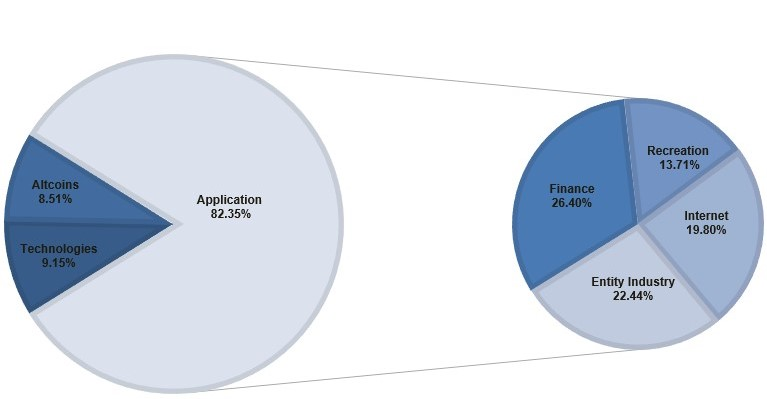
\includegraphics[width=\linewidth]{1}
%\caption{Classification of ICO Projects in 2017}
%\label{fig:1}
%\end{figure*}

The HNB team members include economists, finance and IT professionals, Blockchain technologists and E-commerce entrepreneurs. The key team members have been actively researching and developing Blockchain technologies since 2011. Through in-depth analysis of Blockchain history, technology, economic model and various ICO projects, HNB team has established both its short-term focus and long term foresight of Blockchain. Its short term focus are as follows:

\begin{enumerate}[noitemsep] % [noitemsep] removes whitespace between the items for a compact look
\item  To gain a deep understanding on Blockchain technology and its current status of various applications; 
\item  To point out strategic trend in Blockchain applications and the most critical technological breakthroughs in the field;
\item  To propose HNB’s own economic model, supported both by macroeconomics and monetary theories, including the governance mechanism of the community powered by Blockchain technology;
\item  To utilize the most advanced and mature Blockchain technologies to formulate a technical solution to implement the HNB Blockchain economic model.
\end{enumerate}

%------------------------------------------------

\section{Analysis of Blockchain Economy}

\subsection{\small Current Status of Blockchain Technology and Application}

The first Blockchain was conceptualized by a person (or group of people) known as Satoshi Nakamoto in 2008. It was then implemented the following year by Nakamoto as a core component of the cryptocurrency bitcoin, where it serves as the public ledger for all transactions on the network. In August 2014, the bitcoin Blockchain file size, containing records of all transactions that have occurred on the network, reached 20GB (gigabytes). In January 2015, the size had grown to almost 30GB, and from January 2016 to January 2017, the bitcoin Blockchain grew from 50GB to 100GB in size.

The success of Bitcoin attracts the funding from investment community, According to The State of the Token Market by Fabric Ventures and Token Data, compared to nearly 240 million USD raised by traditional venture investor channels, the total amount of ICOs has exceeded 5.6 billion USD for Blockchain startups spanning a variety of industries. 

There were over 1200 global ICO projects in 2017. According to their business models, they can be roughly categorized into three types (see Figure of Classification of ICO Project in 2017): Technologies (9.15\%), Applications (82.35\%) and Altcoins (8.51\%). After years of development, Blockchain appears to have entered the practical era featured with a variety of innovative applications. People from various industries are rushing into Blockchain field through their own lens and paths, Figure 1. 


\begin{figure}[ht]\centering
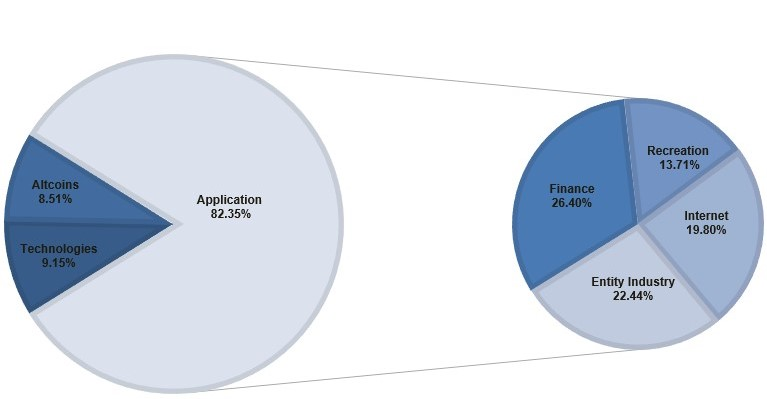
\includegraphics[width=\linewidth]{1}
\caption{Classification of ICO Projects in 2017}
\label{1}
\end{figure}

Speculating on Altcoins potential appreciation seems to create bubbles through ICOs in the cryptocurrency market, it results in the loss of market participant’s confidence in Blockchain applications. The good news is that Altcoins are only made up of less than one tenth of total ICO projects. Statistics shows that (see Figure of Current Status of ICO Projects in 2017) more than 40\% of the ICO projects are sluggish, lost and abandoned. Among 59.3\% of active projects, a considerable portion of them have no real business activities except its minimal maintenance of their websites. According to the State of the Token Market, the success rate of ICO projects is 48\%, Figure 2.


\begin{figure}[ht]\centering
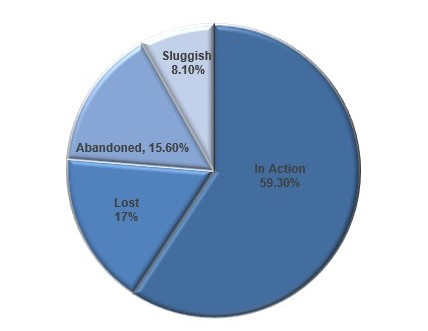
\includegraphics[width=\linewidth]{2}
\caption{Current Status of ICO Projects in 2017}
\label{2}
\end{figure}

The high failure rate among these ICO projects was not only attributed to their dishonest team and unethical behaviors but also largely due to the nature of immatureness of Blockchain technology and its applications. Many Blockchain technologies and economic models are still in their conceptual stages before they can deliver any meaningful and large-scaled applications. 

The market is calling for any breakthroughs on Blockchain technology and innovations on economic or business operating models so that Blockchain application can enter its next level. \\ 

\subsection{Blockchain Development}

HNB team believes that Blockchain develops itself toward three directions in general: 

•   \textbf{Underlying Technology: }Focusing on technical development such as improving TPS to optimize the green consensus mechanism, etc.

•	\textbf{Information Chain: }Making use of Blockchain characteristics such as transparency and tamper-resistance to store key information. For examples, personal credit information, copyright verification and anti-counterfeit, etc.

•	\textbf{Economic Model: }Supporting economic activities on a safer and more efficient Blockchain platform, and continuing to evolve with innovative business operating models.. 

Further interpretations on these three directions of Blockchain development above are as follows:

•	\textbf{For Underlying Technology: }the competition will be so great that no more than ten players would survive. The key to succeed in this direction is technological innovation. In addition, ecosystem construction and economic model implementation are indispensable.

•	\textbf{For Information Chain: }this direction is about Blockchain infrastructure. Information on the chain includes both native information of Blockchain and those beyond Blockchain. It requires tremendous experiments to manage information including storing them in Blockchain, ensuring their authenticity and integrity. Though any lessons learned in this direction will be greatly beneficial to Blockchain development down the road, information chain is difficult to survive because its weak value proposition.

•	\textbf{For Economic Model: }it is believed to be the most promising direction. In any technology evolution, the application is the driver. In Blockchain, however, the economic model plays the leadership role. BTC and ETH are the two most successful Blockchain cases not only because of their technologies but also due to their respective economic models. The successful economic model will generate market demands, and in turn will lead any underlying technologies to be more viable, vital and meaningful.

Based on the viewpoints above, HNB team decide to focus its research on creating an Economic Model built upon Blockchain technology. This paper will present its findings: HNB Blockchain economic model 3.0 and how it is implemented on Blockchain technology backed platform.\\

\subsection{HNB solution for current cryptocurrency limitation}

There have been a large numbers of Blockchain projects based on many economic models in the market, but only BTC and ETH are accepted by the mainstream and be used on a large scale. Figure 3.\\

\begin{figure*}[ht]\centering % Using \begin{figure*} makes the figure take up the entire width of the page
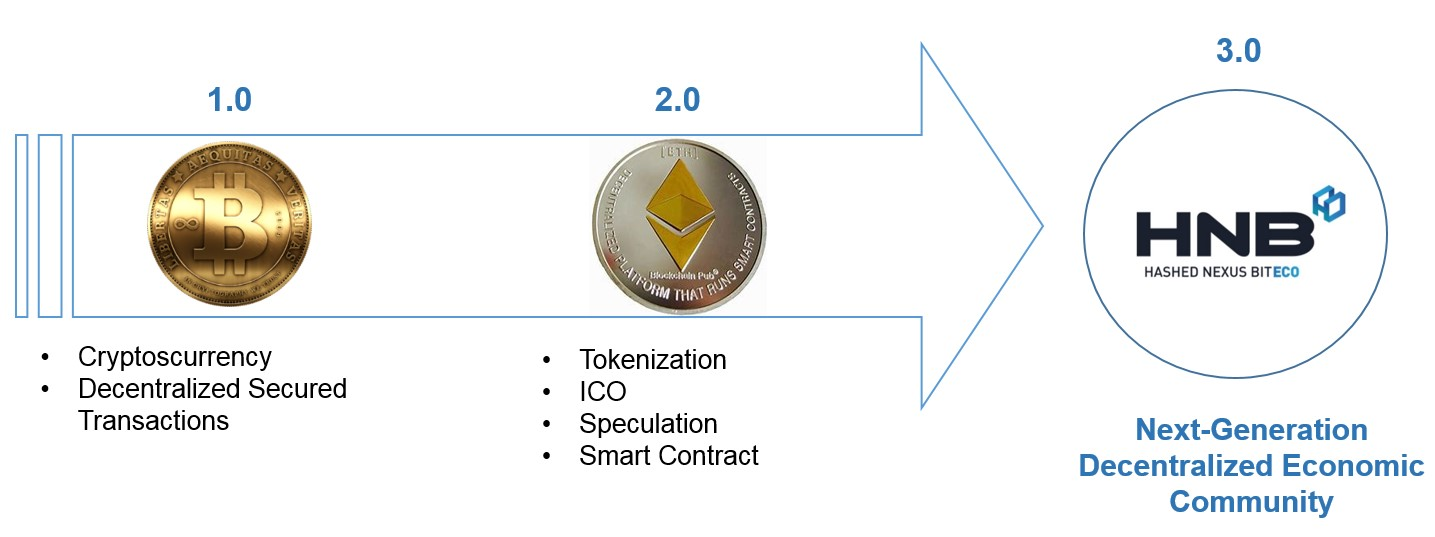
\includegraphics[width=\linewidth]{3}
\caption{Development of Blockchain}
\label{fig:3}
\end{figure*}

\leftline{\textbf {Blockchain 1.0: BTC}}

BTC fulfills the fund transfer function as a crypto asset. It accomplished the fund transfer function in a way that conventional banking can’t - it solves the trust problem between strangers, double-spending pitfall, ensures transparent and immutable transaction information and utilizes distributed ledger that makes it impossible to attack. It is widely used as a digital medium for cross-border fund transfer, currency exchange and even becomes a payment token for some merchants. However, with its limited supply, more and more people regard BTC as a valuable asset rather than “currency” and tend to hold it. As a result, its price has skyrocketed. 

Since BTC is tagged with financial and investment attributes, it has been actively traded in the market resulting in its price volatility, which in turn restrains BTC from being used as stable payment token for any normal business transaction, its acceptance by consumers and merchants is discouraged. For example, Microsoft and Google adopted BTC payment in the earlier years and later discontinued it.

Furthermore, the critical part of BTC transaction flow is that miners are validating the transactions and managing the blocks to gain BTCs as rewards. Currently the transaction fee is 0.0005BTC, it is about 5 USD based on BTC price as of Jan 2018. It was quite high and is even higher if BTC price goes up in the future. The BTC price could be too expensive for users to conduct small fund transfer and would limit the sustainability of BTC economic model. 

Therefore, it can be concluded that it is highly unlikely for BTC to become a commonly-used payment token for goods and services in the future, but to become the universally-agreed valuable asset for preservation and appreciation. \\

\leftline{\textbf {Blockchain 2.0: ETH}}

Built on BTC, ETH is to implement smart contracts functionality, it enables automatic transfer of crypto assets based on any pre-defined rules. With smart contracts, Blockchain is opened up to all sorts of business possibilities. ETH pushes Blockchain application to the new level so that it is recognized as the second milestone in Blockchain after BTC.

Backed by smart contracts, Ethereum can be used in a broad range of application scenarios. For example, it can generate the ERC20 tokens representing various assets and can achieve crypto assets transfer similar to BTC. The most widely used application is ICO that creates a closed-loop trading system (money in and out) so that Blockchain projects can generate ERC20 tokens, raise funds and trade in the exchange market within a short period of time. ICO effective economic model in fact drives Ethereum ecosystem to grow and expand exponentially.

However, ICO economic model has its major flaw. Its sustainability heavily relies on the promise of the token’s potential appreciation. Yet, ICO itself doesn’t create business values. The business value is created by real economic activities. Without any real business transactions, there is limited value in the token. This flaw imposes great uncertainty on the future of Ethereum.
	
Other types of Ethereum application such as information--on-chain, stable currency, decentralized storage and decentralized autonomous organization, are all pure technical solutions but not a closed-loop economic model. Without a value-added economic model, the community will die down over time. Although tokens are still traded in the market, eventually, they will be discarded by investors as these tokens could not generate any real value. 

Blockchain needs an economic model that goes beyond ICO, this model will meet economic needs of people and businesses and help create an economic entity that generate values, invest profits back to the entity to further drive its economic growth, thus forge a closed-loop virtuous economic cycle to self-sustained business generating values in an ever-growing spiral uptrend. Figure 4.\\

\begin{figure}[ht]\centering
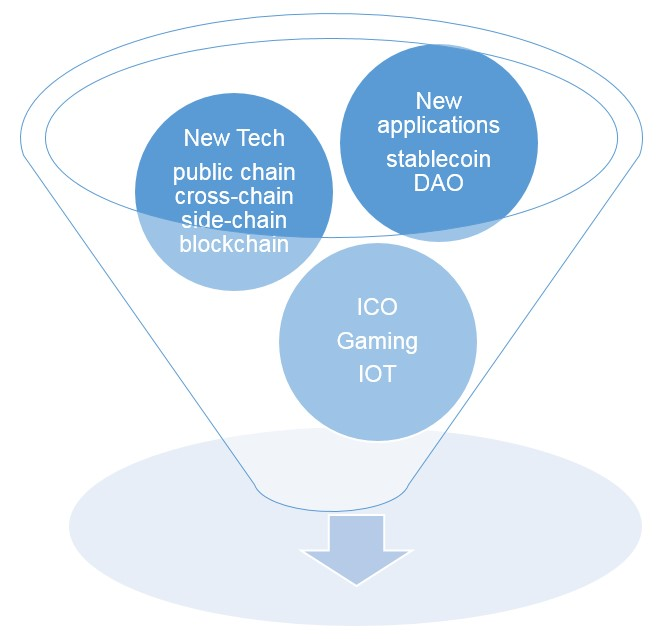
\includegraphics[width=\linewidth]{4}
\caption{}
\label{4}
\end{figure}

\leftline{\textbf {Blockchain 3.0: HNB}}

Standing on the shoulders of BTC and ETH, the next generation of Blockchain applications are looming on the horizon. HNB economic model will embrace the latest Blockchain technologies, integrate with its own innovations, to build a next generation Blockchain based economic entity. The HNB team is confident that its solution will surpass Ethereum and become the next generation of Blockchain milestone application. HNB economic model positions itself as Blockchain 3.0 model.

\begin{itemize}
\item{Economic operation mechanism: Dual-Coin, Asset Token( HNB) and Stable Token ( HGS)}       \item{Community governance: HNB DAO}
\item{Empowered by the latest Blockchain technologies}
\item{Alliance with mainstream brands and merchants}
\item{HNB ecosystem consists of over100 millions of consumers and users.}\\
\end{itemize}


%------------------------------------------------

\section{HNB Economic Model}

\subsection{Mission and Vision}


HNB team are strong believer that Blockchain-based technology and decentralized processes can revolutionize both on-line and off -line market places and commerce. 

HNB mission is to design a Blockchain based economic operation mechanism for a closed-loop economic entity. HNB believes that economic incentives, when transparent and properly implemented, will motivate people to be both active and good participants in the economic entity, if those incentives can be earned throughout the various processes that are running this entity, powered by the communities’ own members. This strengthens the participation and creativity of participants while at the same time allowing the entity to become more dynamic and scalable. 

HNB vision is to follow the footstep of BTC and ETH to be the next generation of Blockchain application. Figure 5.
\begin{figure*}[ht]\centering % Using \begin{figure*} makes the figure take up the entire width of the page
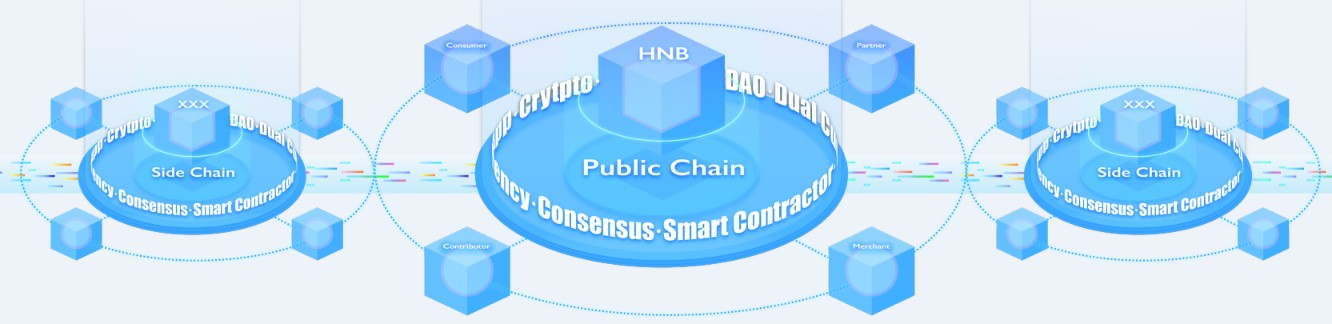
\includegraphics[width=\linewidth]{5}
\caption{}
\label{fig:5}
\end{figure*}

HNB economic entity will deploy a Dual-token system by issuing two types of tokens: Asset Token (HNB Token) and Stable Token (HGS Token): \\

\leftline{\textbf {• HNB Asset Token (“Asset Token” or “HNB Token”)}}

HNB Asset Token is the digital crypto asset representing the ownership of HNB economic entity. Its total supply is fixed to be one billion. Asset Token will be traded on the Cryptocurrency Exchanges. 60\% of HNB Asset Token are distributed among HNB Foundation, HNB team, ecosystem building activities for economic entity and strategic investors. Remaining 40\% are reserved to support the economic development for HNB economic entity.

The intrinsic value of HNB lies in its scarcity and ownership of HNB entity.  For the simple reason that Asset Token stands for asset rights, political rights, property rights and welfare rights in the economic entity, the more prosperous the HNB entity is, the higher value HNB Asset Token will be.\\

\leftline{\textbf {•	HGS Stable Token (“Stable Token” or “HGS")}}

HGS Stable Token is the payment medium (“currency”) pegged with fiat currency like USD. It is issued by “HNB Reserve Committee” and circulated within HNB entity only. HGS Stable Token is used as the medium among social divisions of labor and for trading goods and services. The circulation size of HGS depends on the number of members in HNB entity and its economy (“HNB GDP”). HGS cannot be redeemed or traded in the Cryptocurrency Exchange, only used as payment medium within HNB entity. 

The detailed description of HNB Asset Token and HGS Stable Token is in the following chapters. \\




\subsection{Economic Growth}


\begin{figure}[ht]\centering
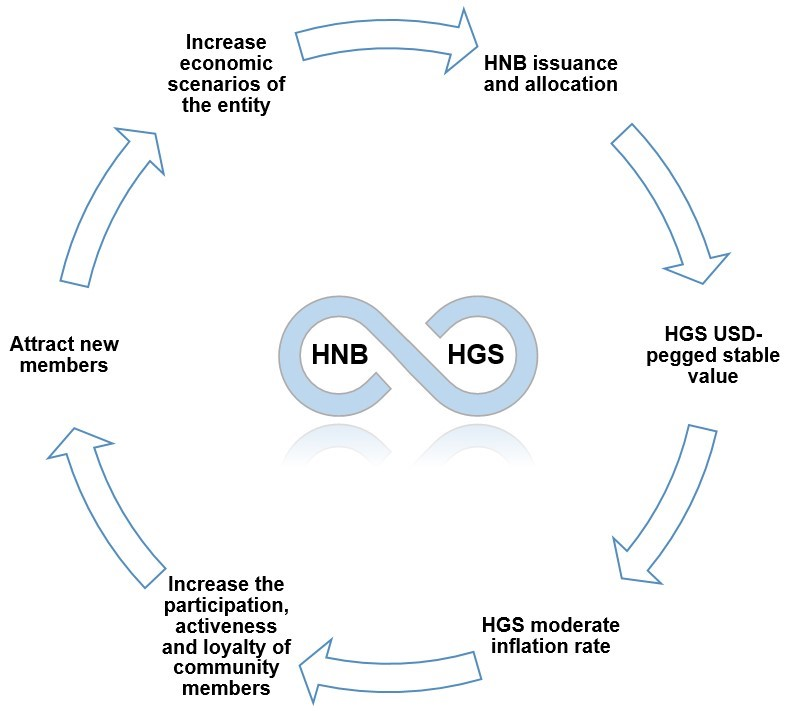
\includegraphics[width=\linewidth]{6}
\caption{Operational Mechanism}
\label{fig:6}
\end{figure}



To safeguard stable economic operation and growth in the HNB community, the operational mechanism, economic policies and governance measures are necessary. Figure 6.\\



\leftline{\textbf {•	Operational Mechanism\\}}

\textbf {HNB Token-Generation, circulation and distribution}

The total numbers of HNB Token are constant. It can be divided into two groups, one group is called Genesis Block generated through pre-mining, accounting for 60\%; another group is generated through mining to support community scale and economic development, accounting for 40\%.

The majority of HNB Token in the first group will be traded at Exchange in the market, except partial lock-in for some holders mandated by smart contracts. The second group of Asset Token will be generated through mining based on certain algorithm in the following 40 years. 

The HNB Token generated from mining, after given as rewards to the miners, is sent to HNB Token (later refer to “Asset Token”) Pool. This pool will be managed by the Token Management Department of HNB community.  Token Management Department functions under the received instructions through community decision-making mechanism, based on the scale and status of HNB economy and in the form of smart contract:
\begin{itemize}
\item{To sell HNB Token to community members through auctions to reclaim HGS;}
\item{To buy back HNB Token through CC Exchange in the community;}
\item{To regulate the circulation of HNB Token in the secondary market.}\\
\end{itemize}



\textbf {HGS Token - generation, circulation, distribution}

HGS Token (later refers to “Stable Token” or “HGS”) Pool managed by Token Management Department initially generates 10 million Genesis blocks prior to pre-mining. Stable Token cannot be traded in the secondary market, instead, it is used as “currency” for products and services within the community. HGS can be used to buy HNB Token through CC Exchange and the Token Management Department within HNB community. 

The	quantities of HGS are not constant, but are determined by the number of community members and its economy size. HGS can also be generated through mining, and then enters HGS token pool and managed by the Token Management Department. This department has following functions:
\begin{itemize}
\item{To manage the HGS supply;}
\item{To reclaim HGS by selling Asset Token or other services.}\\
\end{itemize}

\indent{\textbf {HGS Stable Token-Mechanism}}

HGS adopts regulatory mechanism with its stable value. The mechanism is to ensure HGS to link with fiat currency. It is based on the model of Seignorage Shares with a few additional considerations. Table 1.

 
One of the main usages of digital currency is in consumer-to-business payment markets. However, the payment in the actual scenario has its problem of deflation. Its price fluctuation is too wild to be used for peer-to peer transactions on a daily basis, instead it is treated as a speculative product. In the actual consumption, the monetary aggregate should match the demand and liquidity of the economic system. Effective monetary policies are needed to regulate the relationships between issuance and demand of digital currency. In such an application scenario, we have set a digital currency pegged with fiat currency, regulated by an Algorithm Bank within HNB community.

In current digital currency markets, (as illustrated in the table below), many have proposed solutions to the issues mentioned above. For example, USDT uses fiat currency as collateral and BITCNY/DAI uses digital currency instead. USDT’s solution (using \$USD as collateral) is completely a centralized solution, which is hard to gain trust from everyone, vulnerable to abused activities and even bankruptcy risk.  Collateralization with a fiat currency also increases the potential regulation costs.  BITCNY using digital currency as collateral confronts with wild fluctuation and insolvency of digital currency, therefore it leads to potential trust crisis.

In addition, some emerging digital currencies such as Basecoin regulate the currency value through the algorithm bank based on Seignorage Shares model. The main idea behind this type of digital currencies is to issue the currency based on its supply and demand. Meanwhile, corresponding bonds are issued when its stable digital currency value falls below the pegged fiat currency, users can buy at a lower price of bond, the reclaimed digital currency should be destroyed, and therefore it reduces money supply. The main problem of this model is that if end users loses confidence to the system, they will continue to ask premium to buy the bonds, it will result in deeper discount of bond price and eventually crash whole system. 

\begin{table*}[!ht]
\caption{Comparison between main cryptocurrency}
\centering
\begin{tabular}{lcccccr}
\toprule
Name & Collateral & Form of Collateral & Model & Additional\\
\midrule
USDT & Yes & US Dollar & CDP(Collateralized Debt Position) & N/A \\
BITCNY/DAI & Yes & Digital Currency & CDP & N/A \\
Basecoin & No & No & Seigniorage Shares & N/A \\
HNB Stable Token/HGS & No & No & Seigniorage Shares & Dual Token \\
\bottomrule
\end{tabular}
\label{tab:label}
\end{table*}

HNB community HGS is linked to a fiat currency and calculated based on Seigniorage Shares model. Its supply is subject to the population in the ecosystem and consumption liquidity.  More users including merchants and consumers, etc. are involved in the community, more demands the HGS has. 

As HNB community matures or under certain unforeseen circumstances, a variety of actions will be taken to regulate the currency to maintain its price stability. Auction mechanism is adopted so that it can sell HNB Token to reclaim HGS. Due to the existence of arbitrage space in the auction mechanism, HGS Token will be stable as HNB Token corresponds to the value in the secondary market. In addition, HNB community will work with merchants to generate mutual benefits. For example, certain goods and services are priced at 100 by a fiat currency, and are priced at 96 by HGS, the exchange rate between fiat and HGS is established. The premise for such exchange rate establishment is that it will increase consumers demand while the merchants can gain sufficient profits after discounts. \\

\textbf {Economic Polices}

\textbf{•	Regulatory mechanism for HGS exchange rate with fiat currency and Inflation rate:}
In order to ensure HGS’s price stability, having both stable inflation rate and exchange rate are critical. Any steady economic growth needs these two important economic factors, since their volatility will undermine or even destroy the development of community economy. The targeted inflation rate is to achieve moderate annual inflation (such as 1-3\%), this target range can be maintained through controlling the appropriate size of HGS circulation to match community economic scale. The targeted exchange rate is to peg HGS to fiat currency (such USD) within certain range. The control measure will include “Foreign Reserve Control” in addition to control of HGS circulation within the community. It will manage the volume of exchange and lock the exchange rate within a limited period of time. In the long run, when the economy scale is large enough, the exchange rate will be open, letting market force to determine the exchange rate.\\

\textbf {•	Mechanism for HNB Token price in the secondary market:}
As mentioned above, the Token Management Department can affect HNB Token prices in the secondary market by managing its circulation/supply. \\

\textbf {•	Mechanism for increasing multi layers of economic scenarios:}
HNB community has begun its product and service transactions in 1-2 scenarios, and will gradually introduce more and more scenarios to build a rich, diverse, active and large-scaled economy within the community.  Any sustainable economic community should have followings characteristics:

\begin{enumerate}[noitemsep] % [noitemsep] removes whitespace between the items for a compact look
\item A wide range of economic sectors;
\item Be self-sufficient;
\item Meet the needs of the majority of community members;
\item To reward and attract outsiders to join.
\end{enumerate}

The HNB community can introduce multi-complementary industries and develop them vertically in their own respective value chains. It can also leverage its HNB Token in the form of investment and strategic cooperation to transform an entire ecosystem from the traditional Internet platform to its own Blockchain based community.  To encourage new ecosystems entering the community, the community should have a series of friendly polices to support new participants. \\

\textbf {•	Mechanism for increasing community members’ level of participation, activities and loyalty:}
\begin{enumerate}[noitemsep] % [noitemsep] removes whitespace between the items for a compact look
\item Excellent user experience;
\item Abundant economic scenarios, wealth-creation effect, incentives;
\item Sense of responsibility as the community owners.
\end{enumerate}

\textbf {•	Mechanism for attracting new community members:}
In addition to the aforementioned policies, additional measures and policies will be in place to attract more community members. For example, the policies such as incentives provided by the HNB Token and HGS are expected to attract new members to join. Social contact, newcomer training and other benefits mentioned in following section will also strengthen this mechanism for attaching new community members. \\

\subsection{Collective Value Increase}

In the HNB economic community, there are collective value increases for all community members, Figure 7.

\begin{figure}[ht]\centering
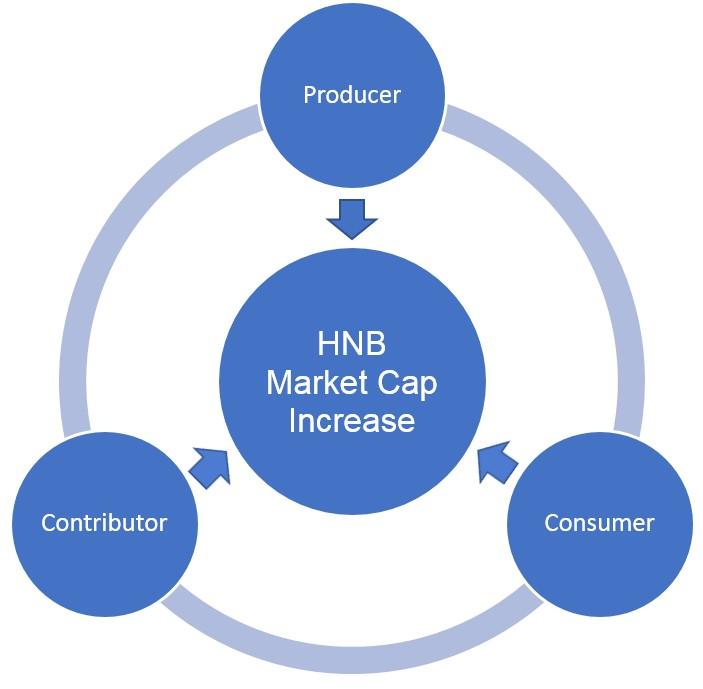
\includegraphics[width=\linewidth]{7}
\caption{Community members and collective value}
\label{fig:7}
\end{figure}

\noindent{\textbf {Producer/Merchant}}
\begin{itemize}
\item{Cost saving --- Cutting transaction costs (by using HGS between merchants and users, avoiding banking costs, hidden costs and more, especially for the repeated business transactions); Higher efficiency of capital/ goods circulation;}
\item{Community-based conflict resolution, by simply majority voting to make decision. (voters are random selected by the system);}
\item{More Income Streams (Rewarding Incentives), in forms of HNB Token and HGS, registered users will receive rewards by participating all events of community, such as voting, clicking advertises, share an opinion or post an article.}
\end{itemize}

\noindent{\textbf {Consumer}}
\begin{itemize}
\item{Buying goods \& services with better price; }
\item{Receiving rewards with HNB Token and HGS by participating all sorts of events in the community;}
\item{Investing HNB Token and being member of HNB community with certain rights \& interests.}
\end{itemize}

\noindent{\textbf {Contributor/Users}}
\begin{itemize}
\item{Promoting products and services; }
\item{Contributing to community events and receiving rewards by participating; }
\item{Investing Asset Token and gaining community rights \& interests. }
\end{itemize}

In building this future, HNB community has the potentials to be the first Blockchain with both real-world business application and mainstream adoption, and may also soon be one of the largest Blockchain networks in existence. \\

%\cleardoublepage
%------------------------------------------------

\section{HNB Governance Framework}

\begin{figure}[ht]\centering
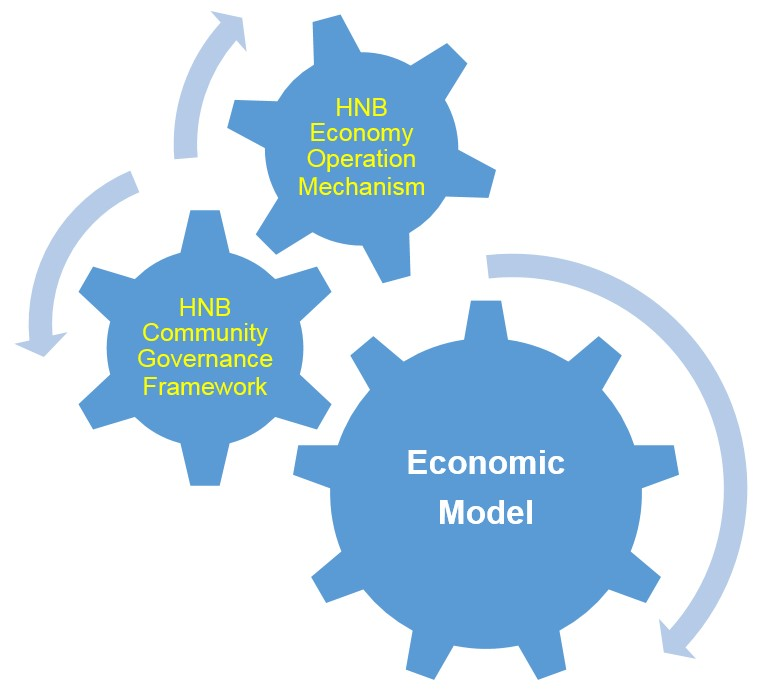
\includegraphics[width=\linewidth]{8}
\caption{HNB Governance Framework}
\label{fig:8}
\end{figure}

While laying the cornerstone of HNB community, HNB team will establish a governance structure to support the self-
development community. HNB team plans to gradually attract and migrate its producers, consumers and contributors into the decentralized community. Once the community reaches a critical mass, be strengthened by incentives provided by both HNB Token and HGS, all governance rights of the community will be handed over to the community members for self-governance. In addition, the HNB team will be dissolved within 24 months after the project is launched. The team members will continue to provide support upon the request of the community, Figure 8.


\subsection{DAO Core Functions(Figure 9)}
The HNB DAO Core Functions include Consensus mechanism (Voting), Incentive/Penalty, Income/Payment, Accounting. These functions are necessary to build an advanced and relatively impeccable community, Figure 10.\\

\begin{figure}[ht]\centering
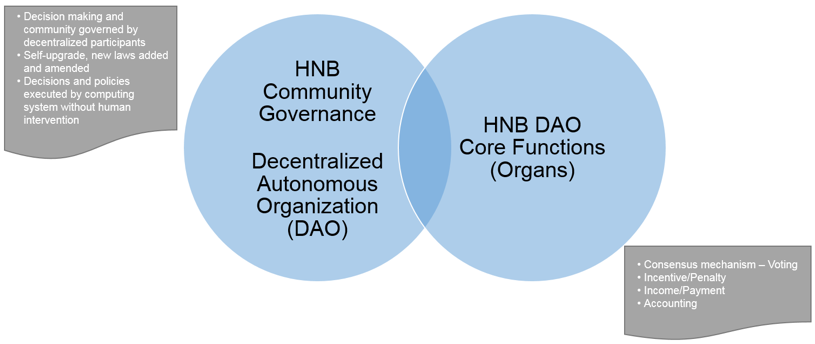
\includegraphics[width=\linewidth]{9}
\caption{DAO Core Functions}
\label{fig:9}
\end{figure}

\leftline{\textbf {•	Consensus mechanism – Voting\\}}
Based on the decentralized autonomous system, HNB Token holders are empowered to play a decisive role in the community governance. When a proposal is approved by more than two thirds of all community HGS Token holders in Community Committee, it will be immediately executed by the smart contracts without any human intervention. Such consensus mechanism will be widely utilized to solve a series of crucial decisions, such as the HGS pricing strategy, on behalf of most community members. If a proposal were not having more than two-thirds of the votes, this proposal would be abandoned. \\

\begin{figure}[ht]\centering
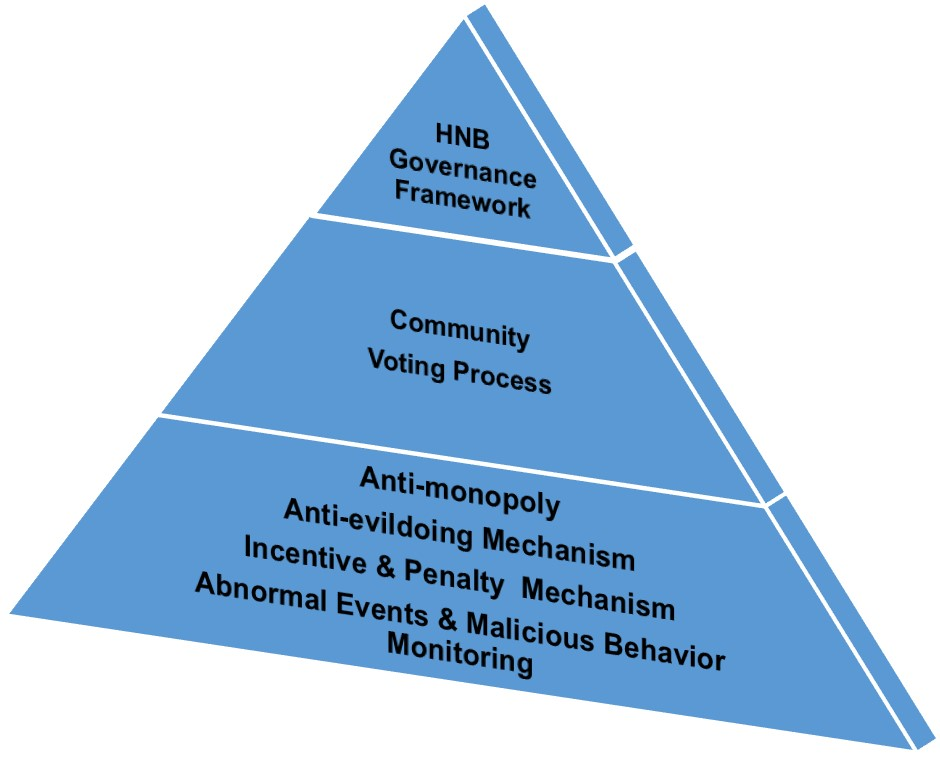
\includegraphics[width=\linewidth]{10}
\caption{}
\label{fig:10}
\end{figure}

\leftline{\textbf {•	Incentive/Penalty \\}}
In the long term, the HNB DAO adopts a series of measures to provide incentive and penalty. Every HNB Token Holder (later interchangeable with term of “HNB community member”) will be granted with the rights to participate all sorts of HNB community events, in return to earn corresponding incomes in recognition of their contributions. Meanwhile, any type of trust breaches or other negative disturbance for community governance must be regulated and be punished via penalty mechanism. Once any disputes emerge, a decentralized arbitration system would enter upon the arbitration process, and make fair jurisdiction to maintain the current stabilization and the further development of the HNB community, by smart contracts. \\ 

\leftline{\textbf{•	Income/Payment}}
Since a myriad of institutions will be actively involved in all aspects of the community, both the HNB Reserve Committee and community members are obliged to offer rewards as incentives to these contributors in recognition of their services provided. This encourages participation and creativity of community members, at the same time fosters the HNB community to be more dynamic, scalable and self-governance. \\

\leftline{\textbf {•	Accounting\\}}
To ensure efficient management of financial resources and effective implementation of community monetary policies, an accounting system is introduced to maintain book-keeping of the whole community. In this way, the cash flow of whole community will be totally open and transparent. Based on the decentralized autonomous organization system, any transactions will be under close public scrutiny. \\


\subsection{DAO Structure}
The overall community governance framework is shown below, Figure 11: 

\begin{figure}[ht]\centering
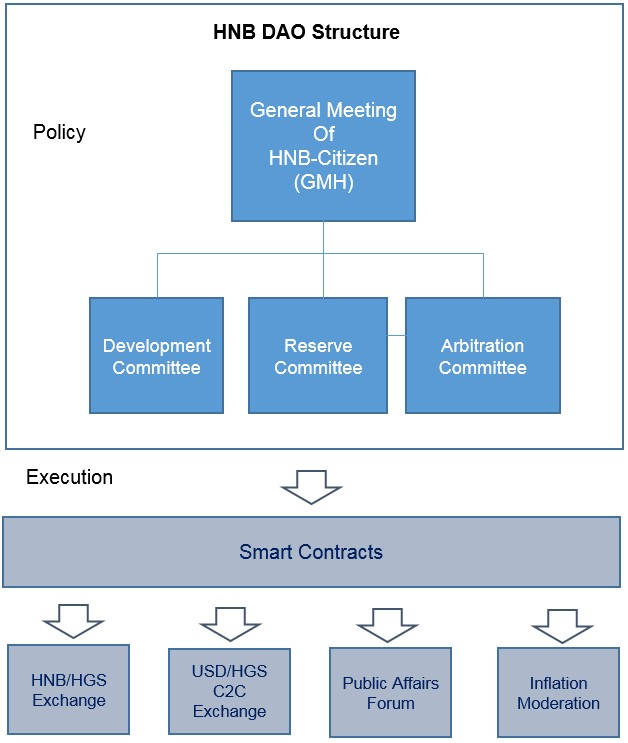
\includegraphics[width=\linewidth]{11}
\caption{DAO Structure}
\label{fig:11}
\end{figure}

\noindent{\textbf {Key features} of the community governance framework}
\begin{itemize}
\item{Policies and Decisions are made by decentralized participants through voting, and executed by smart contracts.}
\item{The most significant affairs are discussed and decided by General Meeting of HNB-Citizen (GMH), such as amending constitution and enacting any new rules, etc. }
\item{Professional committees are elected and appointed by GMH, making policies and decisions under its own delegation of authorization.}
\item{Every policy and decision will be supported by a smart contract, and executed automatically without any human intervention.}
\end{itemize}


\noindent{\textbf {Brief introduction} of each decision-making authority:}

\begin{itemize}
\item{\textbf {General Meeting of HNB-Citizen (GMH)}\\
GMH is the highest decision-making authority in HNB community. It utilizes the number of HNB Token multiply the number of holding days (HNB*DAYs, defined as “Token Age”), to distribute the weight of voting right, governed by means of Proof of Stake (POS). With any significant issues, only the proposal having more than 2/3 votes will be valid and executed accordingly. }
\item{\textbf {Development Committee}\\
Development Committee is under the authorization of the GMH, it is responsible for HNB community daily routines under its sole discretion. The committee is made of a team of elected representatives, with a team leader who takes responsibility of making any final decisions. The Committee will take on coding and co-chain of all matters under the GMH, and will ensure smart contracts to be executed automatically. Community representatives are selected based on factors such as “HNB Token Age” and the numbers of votes cast, and are subject to replacement at any time according to community members voting result. Three factors are weighted in this process: \\
1)	The number of Tokens held – objective; \\
2)	The days that the token is held – objective; \\
3)	The number of votes cast – subjective. \\
}
\item{\textbf {Reserve Committee}\\
Reserve Committee is responsible for two accounts holding: HNB Token and HGS. Under direction of the General Meeting of HNB-Citizen (GMH), the Reserve Committee adopts a series of “token policies” and take charge of various economic operation as followings:
1)	Paying HGS to any community contributors; \\
2)	Facilitating any exchange between HNB Token and HGS; \\
3)	Maintaining Stable Token’s inflation rate and exchange rate between Stable Token and fiat currency (such as USD). \\
4)	Regulating Asset Token price at the secondary market through adjusting its circulation to ensure the community development in smooth and steady manner. \\}

\item{\textbf {Arbitration Committee}\\
As a relatively independent committee appointed by GMH, Arbitration Committee is in charge of solving disputes among community members. During arbitration, corresponding deposits (in form of Tokens) from both sides should be frozen until verdict is reached. To ensure the fairness and impartiality, the procedure would be executed by cryptographic algorithm and judgements among judges remain independent and confidential. Once the arbitration verdict is reached, smart contracts would carry out compensations or punishments to litigants. The arbitration committee would charge the losing party a reasonable fee to support long-term operation of the committee.}\\

\item{\textbf {Incentive and punishment mechanisms}\\
HNB community adopts comprehensive Incentive and punishment mechanisms to regulate the election of GMH to ensure fairness and openness. To avoid electoral frauds, One principle and one measurement is adopted as follows:
\begin{enumerate}[noitemsep] % [noitemsep] removes whitespace between the items for a compact look
\item \textbf{Majority principle:} the decisions must be accepted by majority of the community members, i.e. 2/3 member’s votes will pass and execute any proposal. 
\item \textbf{BPFT (Practical Byzantine Fault Tolerance) Algorithm:} the consensus mechanism is supported by BPFT Algorithm, to implement the general voting. 
\end{enumerate}
}

\item{\textbf {Punishment mechanism}\\
If any representative abuses the power such as seeking personal gains, the punishment will be imposed in two ways.
\begin{enumerate}[noitemsep] % [noitemsep] removes whitespace between the items for a compact look
\item All possessions in the account would be confiscated. 
\item The membership would be evicted from HNB community and be prohibited from re-entering.
\end{enumerate}
}
\end{itemize}

To motivate the community members to vote, HNB community embraces following three mechanisms:\\

\noindent{\textbf {Incentive mechanism: }}
Any voters will be rewarded by voting. When voters turn out to be on the majority side and the proposal is accepted, they would be rewarded twice as many as the original bets/deposits for attending. If the voters were on minority side, they would lose all their rewards as well as original deposits.

\noindent{\textbf {Blind vote mechanism: }}
To encourage the community members to make the right decisions, HNB community forbids any sorts of communication among voters and voters will not have any access to other’s decision until the final results is revealed. 

\noindent{\textbf {Constitution regulation: }}
All voting procedures must comply with HNB community constitution.


\subsection{Community Operations Mechanism}

HNB community economic operation framework is shown below, Figure 12: \\

\begin{figure*}[ht]\centering % Using \begin{figure*} makes the figure take up the entire width of the page
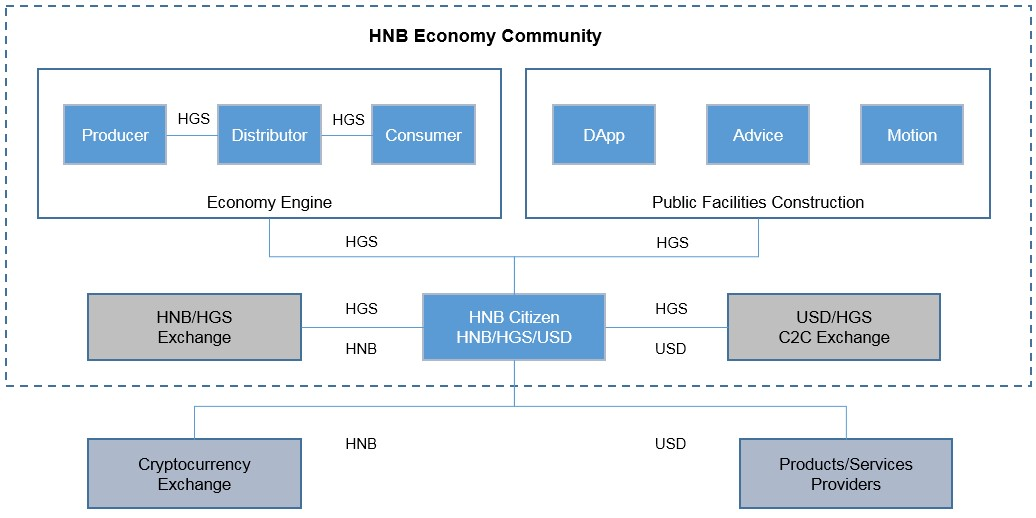
\includegraphics[width=\linewidth]{12}
\caption{Community Operations Mechanism}
\label{fig:12}
\end{figure*}


\noindent{\textbf {•	HNB community members (interchangeable with “HNB Citizen”) can earn HGS through working, such as creating values in Economic Engine or participating in Public Facilities Construction.  }

Economic Engine section illustrated in the chart above, HGS is circulated among producers, distributers and consumers. All participants in HNB community will enjoy their respective benefits of being HNB Citizens. Producers and distributers are rewarded with HGS through a series of economic activities. On the other hand, customers in HNB community can use HGS, through exchange with FIAT, to engage business transactions and to invest on HNB Token for potential value appreciation. \\}

\noindent{\textbf {•	HNB Citizen can invest HNB Token using HGS on Exchange within HNB community. HNB/HGS Exchange is operated based on the algorithm set up by HNB Reserve Committee. }

The most promising investment of using HGS in HNB community is to invest in HGS Token for its’ potential value appreciation. \\}

\noindent{\textbf {•	HNB Citizen can inter-exchange USD with HGS in USD/Stable Token C2C Exchange, a DApp on HNB Chain. }}

Each member can inter-exchange USD or other fiat currency via the C2C Exchange platform at relatively fixed rate, and then use HGS to conduct business transaction as desired. \\

\noindent{\textbf {•	 HNB Citizen can trade HNB token at Cryptocurrency exchanges to other cryptocurrencies or fiat currency e.g USD outside of HNB community.}}

USD is a bridge for HNB Token and other cryptocurrencies to link with conventional economy. \\

%-----------------------------------------------

\section{HNB Application Scenarios}


\noindent{\textbf {Cultural Recreation – Honey}}

HNB team has been working with the world’s largest hand-painted IP platform called Honey. With more than 100,000 artists and 30 million users, Honey helps users paint the cartoon portraits through Internet. At present, more than 95\% of celebrities in China as well as many celebrities from United States, Japan and South Korea, etc. are Honey’s customers.

Honey launched a KOL fan realization tool, a small program on WeChat platform, to help run its own painting business and sell peripheral products. By leveraging WeChat, one of the world’s largest social network platform with one billion+ users, Honey’s KOL fan realization tool can have great potentials to extend its user base. Currently HNB Token/HGS payment have been implemented in KOL so that users can pay KOL services by using HGS, Figure 13.

\begin{figure}[ht]\centering

\includegraphics[width=\linewidth]{13}
\caption{Cultural Recreation – Honey}
\label{fig:13}
\end{figure}

There are number of pain points for Honey. For example, Honey lacks an effective copyright Protection system for hand painting especially the intangible digital products. 

With Honey becoming more and more successful, its legal expense would be dramatically increased while more competitors would be threats to its IP. By migrating into HNB community, backed by Blockchain technologies, Honey’s costs would be reduced and its IP would be protected.\\


\noindent{\textbf {Commodity – Longmi}}

Longmi is the top brand in China selling rice products through multi-channels including on the Internet. It currently has one million customers with an annual growth rate of 200\%. Longmi launched a new brand - Jinaling, to sell rice products through WeChat.  HNB/HGS payment has been implemented in Longmi sale platform. Figure 14 and Figure 15.

\begin{figure}[ht]\centering

\includegraphics[width=\linewidth]{14}
\caption{Commodity – Longmi}
\label{fig:14}
\end{figure}

\begin{figure}[ht]\centering
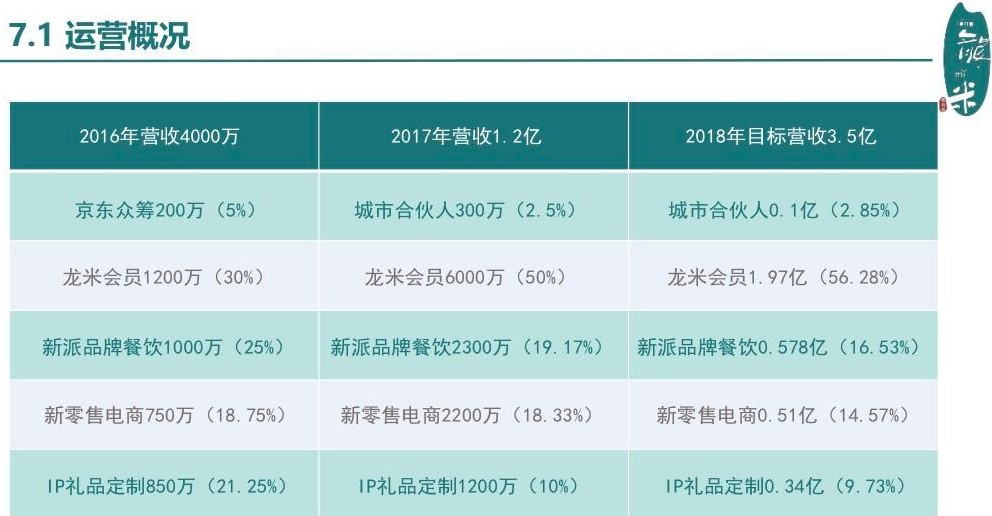
\includegraphics[width=\linewidth]{15}
\caption{}
\label{fig:15}
\end{figure}

Rice market is open to all in China so Longmi is faced with a challenge to deal with counterfeit products in the marketplace.  By migrating into HNB community, backed by Blockchain technologies, Longmi could effectively protect its brand and grow its business. \\

\noindent{\textbf {Health \& Agriculture – Uncle Bull}}

\begin{figure}[ht]\centering
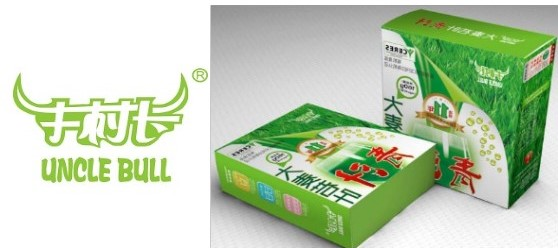
\includegraphics[width=\linewidth]{16}
\caption{Health \& Agriculture – Uncle Bull}
\label{fig:16}
\end{figure}


Uncle Bull is an online e-commerce company selling organic green food. It covers 1000+ eVendors, 2000+ Supermarkets and 400K+ members. HNB/HGS payment has been implemented in Uncle Bull platform, Figure 16.

By migrating into HNB community, backed by Blockchain technologies, Uncle Bull could effectively address the following challenges.
\begin{itemize}
\item{Product management by Blockchain technologies. }
\item{Vendor dispute management by HNB community conflict resolution}
\item{•	With merchants clamoring to lower their cost of accepting payments through HGS, the consumers-to-business payment markets ( with its multiple high profitable intermediaries ) provides a straightforward use case for a decentralized ledger}
\end{itemize}


%------------------------------------------------

\section{HNB Technical Solution}

HNB platform has many of its own innovations that adopts the cutting-edge theories, technologies from the current Blockchain initiatives and projects in the market 

The uniqueness of HNB project is to establish a decentralized economic model based on public Blockchain. The followings are the factors for HNB technical architecture design, its business ambition and its sustainable growth.

\begin{itemize}
\item{\textbf {Scalability:} support continuous HNB community growth}
\item{\textbf {Performance:} support millions of users and concurrent transactions}
\item{\textbf {Security:} strong security at application and infrastructure level}
\item{\textbf {Interoperability:} support easy integration with existing systems and ongoing development}
\end{itemize}

The key features of HNB technical solution includes:
\begin{itemize}
\item{One public chain for Dual-Token: HNB and HGS}
\item{Regulatory mechanism for HGS price stability}
\item{Innovative consensus mechanism}
\item{Supports smart contracts}
\item{Robust Organic DApp Collection, such as:\\
o	Decentralized trading platform\\
o	Decentralized auction platform\\
o	Decentralized digital currency/fiat currency exchange platform
}
\item{Strong Security \& Encryption}
\item{High Performance and scalability}
\end{itemize}


\subsection{Architecture}

HNB architecture follows a design philosophy that includes layers-based approach, modular extension, interoperability, and emphasis on performance and security, Figure 17.

\begin{figure}[ht]\centering
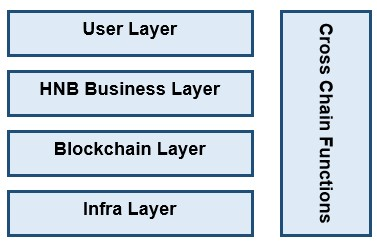
\includegraphics[width=\linewidth]{18}
\caption{}
\label{fig:18}
\end{figure}

HNB technical architecture defines the structure and interaction of the platform services, user oriented layer, HNB public chain business functions and supporting components based on mainstream Blockchain technologies.

\begin{itemize}
\item{User Layer}
\item{Business Layer – HNB Business Services}
\item{Core Layer – HNB Core Blockchain}
\item{Infrastructure Layer}
\item{Cross-Layer Functions }
\end{itemize}



The detailed view of the HNB architecture and core building blocks are illustrated in the Figure 18.

\begin{figure*}[ht]\centering % Using \begin{figure*} makes the figure take up the entire width of the page
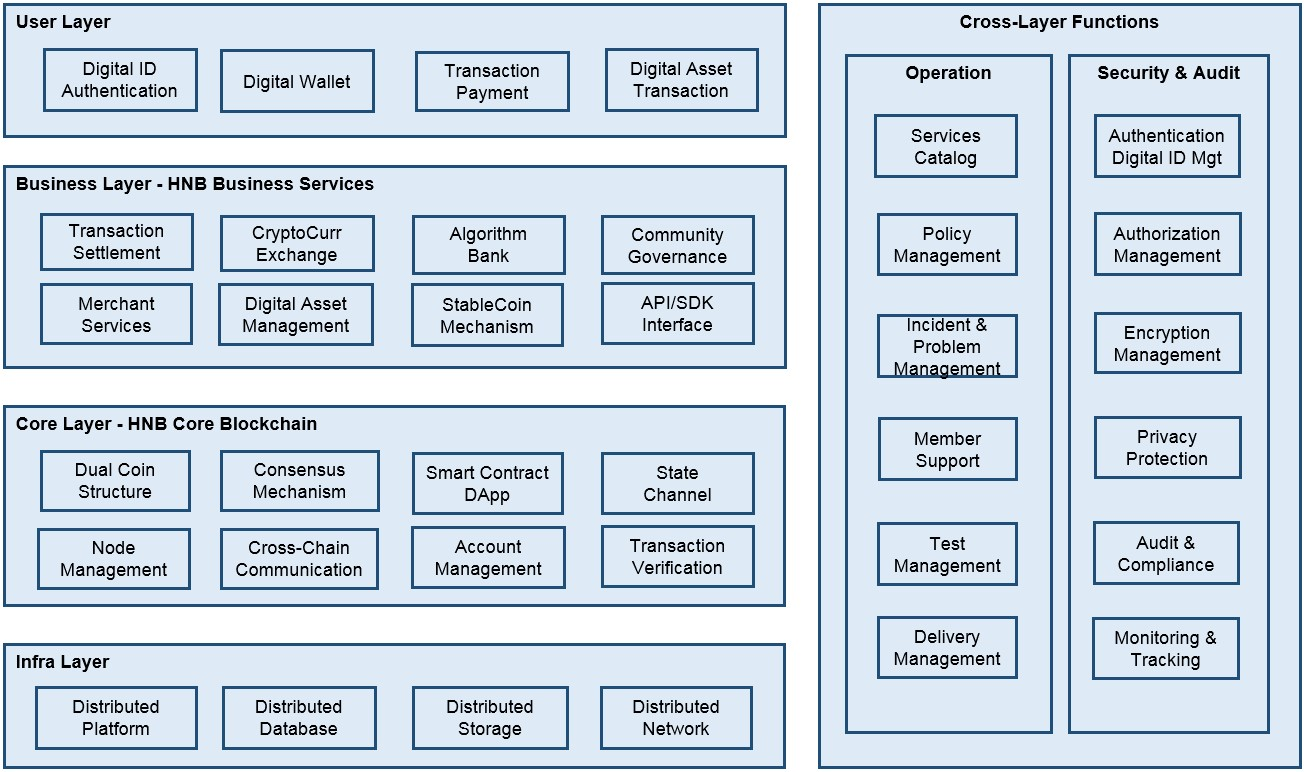
\includegraphics[width=\linewidth]{19}
\caption{Detailed view of the HNB architecture and core building blocks}
\label{fig:19}
\end{figure*}

\subsection{Functions by Layer}

\underline{\textbf {User Layer}}

User layer is the entry point for end users. Users access HNB Blockchain services via the user layer.
From technical perspective, some of these front-end features are supported by HNB’s DApp services, which will be described in chapter 6.4 DApp infrastructure.\\

\textbf {•	Digital ID Authentication(Figure 19)}

\begin{figure}[ht]\centering

\includegraphics[width=\linewidth]{20}
\caption{Digital ID Authentication}
\label{fig:20}
\end{figure}

User can register the membership of HNB Blockchain to join the community. Two types of user onboarding process are supported:

o	New users to HNB economic community

o	Existing users from HNB business partners in the ecosystem 

During the registration process, HNB backend Digital ID service module will generate the public key and private key pair for the user; and HNB CA (Certification Authority) services will generate and sign the certification following X.509 standard based on public key as user’s digital ID for future transactions and activities in the community.

The overall process shows as the follow diagram. Figure 20.

\begin{figure*}[!hpbt]\centering % Using \begin{figure*} makes the figure take up the entire width of the page
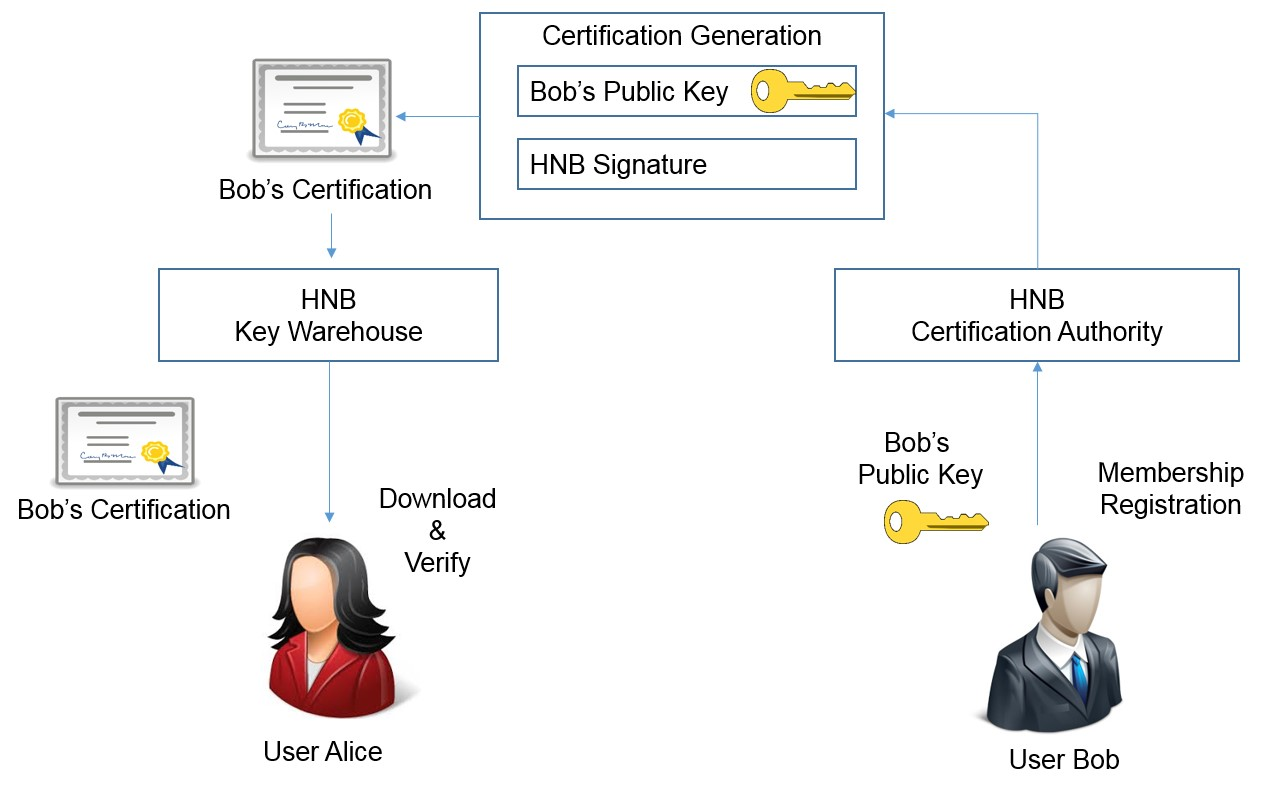
\includegraphics[width=\linewidth]{21}
\caption{the overall process}
\label{fig:21}
\end{figure*}

After the registration process is completed, users will be assigned with the default roles in the HNB community. \\

\textbf {•	Digital Wallet}

Digital Wallet provides the user interface to manage various cryptocurrencies and digital assets. It serves as an entrance to a series of DApps (decentralized applications) constructed on HNB Blockchain, Figure 21. \\


\begin{figure}[ht]\centering
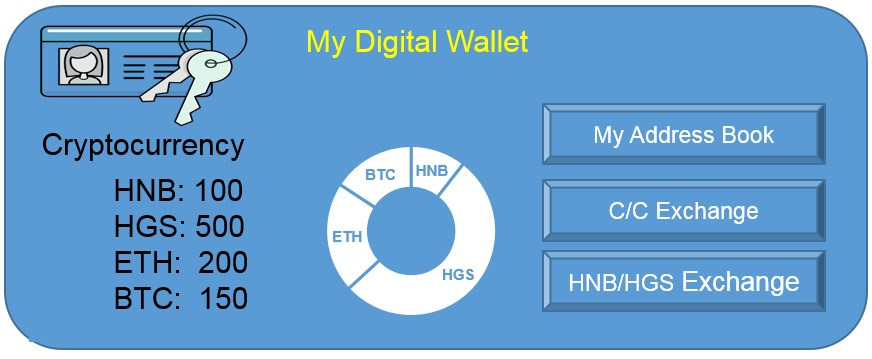
\includegraphics[width=\linewidth]{22}
\caption{Digital Wallet}
\label{fig:22}
\end{figure}

With the digital wallet, users can hold and protect cryptocurrencies. At the same time, user can deal with a variety of crypto-assets that have been developed in HNB community. \\

\textbf {•	Transaction Payment}

User can perform various goods and services payment transactions in HNB community via HGS (Stable Token as medium currency). \\

\textbf {•	Digital Asset Transaction}

It links users to HNB services such as C2C - Customer to Customer (or OTC - Over the Counter Market), C/C Exchange (for exchange with other cryptocurrencies) and Fiat current/HGS C2C Exchange. \\

\textbf {•	Community Hall}

User can participate in HNB community forum, secure their own position for relevant incentive program, air-drop, discuss and vote for community policy, governance motion, information billboard etc. and other community’s events. \\ 

\noindent{\underline{\textbf {Business Layer - HNB Business Services}}}

HNB Business Services layer realizes all core business logics of HNB decentralized economic community.

From technical perspective, some of these features are supported by HNB’s DApp services, which will be described in chapter 6.4 DApp infrastructure. \\

\textbf {•	Transaction Settlement}

Transaction settlement supports various goods and services transactions occurred in the community among consumers and producers. 

Transaction details will be encrypted and stored securely in HNB central database. The hash value of each transaction details will be stored as key to search the transaction for traceability.

Account balance change transactions will be sent to core Blockchain layer to be validated and published to the HNB public Blockchain based on HNB’s innovative consensus mechanism. \\

\textbf {•	Merchant Services}

Merchant Services is a platform to support merchants/producers’ sales promotion campaigns and auctions.

The services can be realized by DApps for merchants/producers easy plan, deployment, launch and management of products and services sales and promotion/discount policies. 

It can also support seamless integration with existing merchants/producers’ e-commerce websites, and the transaction will be conducted via HNB Blockchain. \\

\textbf {•	Cryptocurrency Exchange}

CyrptoCurr Exchange supports HNB Token exchange with other mainstream cryptocurrencies in the market such as ETH, BTC, EOS, etc. \\

\textbf {•	Digital Asset Management}

Corresponding to the digital asset transaction in the user layer, it provides the backend supports. Digital Asset includes future new digital assets created and circulated in HNB community. \\

\textbf {•	Algorithm Bank}

The purpose of Algorithm Bank is to define and publish HNB economic development policies based on all-aspect parameters of HNB community populations, transaction volumes, CPI, etc. The output of the policy could be, HNB issuance, HGS issuance, inflation adjustment measures, investment for community construction facilities, etc.

Algorithm Bank acts as central bank in real economy, but it’s based on the algorithm designed by HNB community. Expanding and contracting the money supply works because the Quantity Theory of Money states that long-run prices in an economy are proportional to the total supply of money in circulation.

Further illustration about HNB Algorithm Bank through future series of white paper with focus on economic sustainable growth model will be published. \\
 
\textbf {•	Stable Token Mechanism}

HNB architecture realizes Dual Token system, HNB Token as Asset Token and HGS as USD-pegged /CPI-pegged Stable Token.

The core of the Stable Token Mechanism is to support how HNB Blockchain tightens and easing HGS supply to maintain its price stability. 

o	The mechanism defines peg based on USD and Consumer Price Index (CPI) - a basket of goods and services trading in HNB community

o	It defines a target price for HGS in the combined pegged assets

o	HNB Blockchain monitors exchange rate to measure price via a specific prediction systems in a decentralized way

o	HNB Algorithm Bank expands and contracts the supply of HGB in response to deviations of the exchange rate from the peg.

More white papers with focus on Stable Token mechanism based on HNB market research will be published on its web site www.hnb.eco.  \\

\textbf {•	Community Governance}

Its process is laid out in the chapter of HNB Governance Framework. \\

\textbf {•	API/SDK Interface}

APIs and SDK (Software Development Kit) enables HNB community members/contributors/developers and other applications to interface with HNB.

Details will be published and updated in future HNB web site www.hnb.eco and Github. \\


\noindent{\underline{\textbf {Core Layer - HNB Core Blockchain}}}

\textbf {•	Dual Token Structure}

HNB dual token structure will be explained in details in the chapter of 6.2 on Public Chain Design. \\

\textbf {•	Node Management}

Node refers to the computer system connected to HNB Blockchain. It is a critical aspect of cryptocurrency protocols. Along with mining, unit quantity caps, and anti-double spending security, nodes are playing one of the most important roles in any cryptocurrency. Both full node and light node are equally important. 

Full nodes provide the complete history and preserve it as a failsafe in case the cryptocurrency network is unavailable. Light nodes perform functions that support cryptocurrencies when the entire Blockchain history is not needed. People who maintain nodes, together with people who mine cryptocurrencies provide essential services. Without them, cryptocurrencies would not be able to function properly.

HNB supports Full Node, SPV (Simplified Payment Verification) node and mining node, Figure 22. \\


\begin{figure}[ht]\centering % Using \begin{figure*} makes the figure take up the entire width of the page
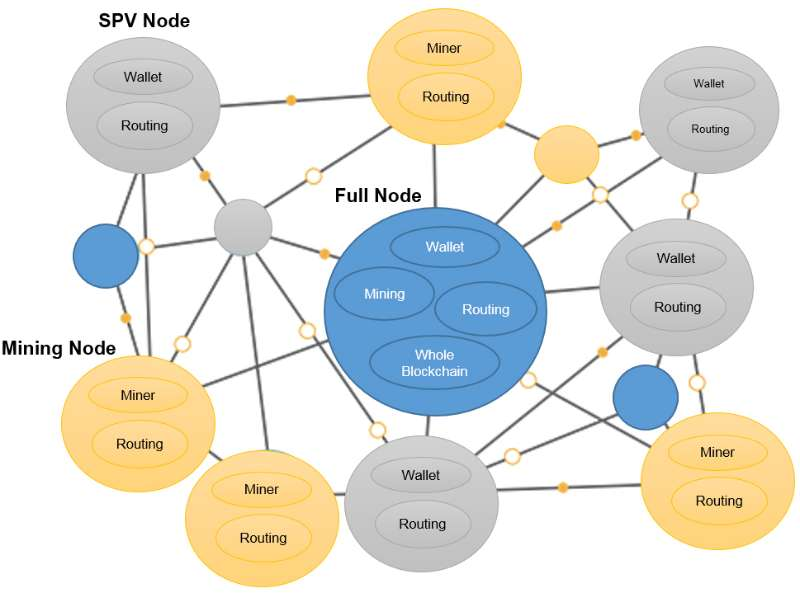
\includegraphics[width=\linewidth]{39}
\caption{Node Management}
\label{fig:23}
\end{figure}
Node management supports HNB public chain mining and node incentive \& penalty mechanism. Incentives must be rewarded to the participating nodes who follow the regulation, while punishments must be imposed to the violators, so as to allow the whole system to work in a virtuous circle.

Other management features include:

o	Node information and status query

o	Node Configuration Management

o	Node Network Connection Monitoring

Node Authorization management. \\

\textbf {•	Consensus Mechanism}

HNB Dual Token structure will be explained in details in the chapter of 6.3 on Consensus Mechanism. \\

\textbf {•	Cross-Chain Communication}

One consideration on design is to define the communication between HNB public chain and the future sidechains in the HNB community.

The side chain can be used for a specific business model and operation for HNB community producers and contributors. Alternative cryptocurrencies and digital assets could be issued in side chain.

Multi-coin Smart Contract will be used to support data exchange between HNB public chain and its side chains. For example, the smart contract codes on HNB public chain are programmed to verify the consensus finality of events on side chains directly. \\

\textbf {•	Smart Contract/DApp}

HNB Smart Contract/DApp will be explained in details in the chapter of 6.4 on DApps. \\

\textbf {•	Account Management(Table 2)}

In HNB Blockchain, there are two types of accounts: Externally owned accounts and Contracts accounts.\\

\begin{table*}[hbt]
\caption{Account Management}
\centering
\begin{tabular}{lp{4cm}p{8cm}p{14cm}r}
\toprule
Account Type & Brief Definition & Key Points \\
\midrule
Externally
Owned
Accounts
 & 
An externally owned account (EOA) is also known as an account controlled by a pair of private keys, which may be held by a person or an external server or other trusted endpoints.
 & 
\begin{itemize}
\item{Contains a balance of HNB/HGS}
\item{Capable of sending transactions}
\item{Controlled by the account’s private keys}
\item{The public/private key pair is generated when user registers a new account with HNB}
\item{Has no code associated with it}
\end{itemize}
\\
\midrule
Contracts
Accounts
 & 
Contract accounts are not controlled by people. They store instructions and are activated by external accounts or other contract accounts.
 & 
\begin{itemize}
\item{Have an HNB/HGS balance}
\item{Hold some contract code in memory}
\item{Can be triggered by people (sending a transaction) or other contracts sending a message
}   \item{When executed, can perform complex operations}
\item{Have their own persistent state and can call other contracts}
\end{itemize}
\\
\bottomrule
\end{tabular}
\label{tab:label}
\begin{flushleft}
o	\textbf{An account} is a data object, an entry in the Blockchain ledger, indexed by its address, containing data about the state of that account, such as its balance.\\
o	\textbf{An address} is a public key belonging to a particular user. It’s for users to access their accounts. It is technically the hash of a public key. \\
\end{flushleft}
\end{table*}


\textbf {•	State Channel(Figure 23)}

\begin{figure}[ht]\centering % Using \begin{figure*} makes the figure take up the entire width of the page
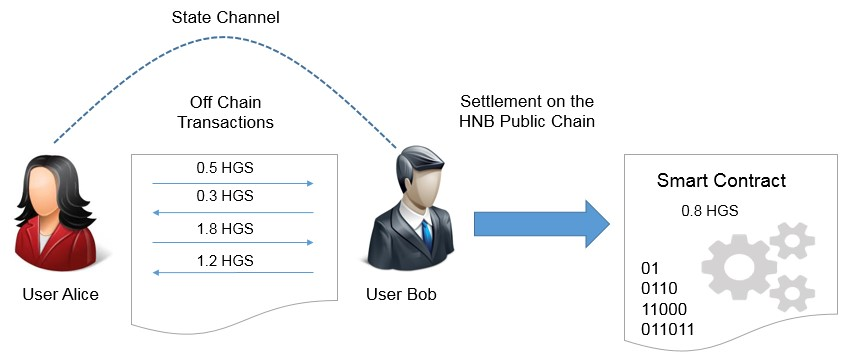
\includegraphics[width=\linewidth]{24}
\caption{State Channel}
\label{fig:24}
\end{figure}

State Channel is the approach proposed for speeding up the transaction on HNB Blockchain network. The basic idea is to use side channels for state updating and processing transactions off the main chain. Once the state is finalized, it is written back to the main chain, thus offloading the time-consuming operations from the main Blockchain, Figure 23. 

State channel works by performing the following three steps:

o	First, a part of the Blockchain state is locked under a smart contract, ensuring the agreement and business logic between participants. 

o	Then off-chain transaction processing and interaction start between the participants who only update the state between themselves. In this step, almost any number of transactions can be performed without the Blockchain that makes the process fast and a best candidate for solving Blockchain scalability issues. 

o	Once the final state is reached, the state channel is closed and the final state is written back to the main Blockchain. And then the locked part of the Blockchain will be unlocked.\\

\textbf {•	Transaction Verification}

Transaction is the fundamental part of a Blockchain. A transaction represents a transfer of value from
one address to another.

Any transactions posted from nodes on the Blockchain are verified based on a predetermined set of rules and only valid transactions are selected for inclusion in a block.

Transaction verification rules, such as:

o	Check the syntax and ensure that the syntax of the transaction is correct.

o	Verify that inputs and outputs are not empty.

o	The output value must be in the allowed money range

o	For each input, there must exist a referenced output transaction

o	Reject nonstandard transactions

Block validation is to check the coherence of the cryptographic signature of the block with the history stored in the entire Blockchain. Block finalization is a process run by miners in order to validate the content of the block and apply rewards(See in Table 3).\\

\begin{table*}[!hbpt]
\caption{Infrastructure Layer}
\centering
\begin{tabular}{lp{13cm}p{10cm}r}
\toprule
Distributed Network
 & 
\begin{itemize}
\item{HNB public chain runs over (P2P) Peer to Peer network on top of Internet}
\item{Nodes communication over Transport Layer Security (TLS) for security}
\end{itemize}\\
\midrule
Distributed Platform
 & 
\begin{itemize}
\item{HNB consists of thousands of nodes running HNB client system}
\item{Node in HNB Blockchain network perform various functions depending on the role it plays such as full node, lightweight node, etc.}
\end{itemize}\\
\midrule
Distributed Storage & 
\begin{itemize}
\item{Decentralized file system based on IPFS (Inter Planetary File System)}
\item{HNB client system that runs on the nodes and connects to the peer-to-peer network from where Blockchain software is downloaded and stored locally}
\item{All users of the HNB Blockchain maintain a copy of the ledger on their local nodes and use a distributed consensus mechanism in order to reach a decision about the eventual state of the ledger}
\end{itemize}
\\
\midrule
Distributed Database
 & 
\begin{itemize}
\item{Decentralized key-value database at node level}
\item{Support RethinkDB/MongoDB/LevelDB}
\end{itemize}
\\
\bottomrule
\end{tabular}
\label{tab:label}
\end{table*}

\noindent{\underline{\textbf {Cross-Layer Functions}}}\\
Cross-Layer Function is classified in two categories: \textbf {Operation, Table 4} and \textbf {Security \& Audit, Table 5}.

\begin{table*}[!hbt]
\caption{Operation}
\centering
\begin{tabular}{lp{10cm}p{50cm}r}
\toprule
Services Catalog
 & 
\begin{itemize}
\item{List of services provided in HNB Community including public chain and sidechains}
\item{Services support info, technical info and documentation}
\end{itemize}\\
\midrule
Policy Management
 & 
\begin{itemize}
\item{Responsible for policy management of various policies specified in HNB system, such as the voting policy, consensus policy, or group management policy. }
\item{It interfaces and depends on other modules to enforce the various policies. }
\end{itemize}\\
\midrule
Incident \& Problem Management
 & 
\begin{itemize}
\item{Provide the function for systems monitoring including abnormal events and transactions, potential malicious node behaviors, security threats and attack at application level and network infrastructure, etc.}
\item{Deploy the mechanism for incident management, emergency response process}
\item{Problem Management is the process responsible for managing the lifecycle of all problems. The primary objectives of Problem Management are to prevent problems and resulting incidents from happening, to eliminate recurring incidents and to minimize the impact of incidents that cannot be prevented.}
\end{itemize}
\\
\midrule
Member Support
 & 
\begin{itemize}
\item{Track and manage support requests from HNB community members}
\end{itemize}
\\
\midrule
Test Management
 & 
\begin{itemize}
\item{Management process and tools across the full HNB application lifecycle, including testing, deployment, updates, and decommissioning of obsolete features. }
\item{Test blockchain is used to test smart contracts and DApps before being deployed to the production live blockchain. }
\item{Establish test environment, test process and documentation. }
\end{itemize}\\
\midrule
Delivery Management
 & 
\begin{itemize}
\item{Management process and tools across the full HNB application lifecycle, including testing, deployment, updates, and decommissioning of obsolete features }
\item{Release/Version Management }
\end{itemize}\\
\bottomrule
\end{tabular}
\label{tab:label}
\end{table*}


\begin{table*}[!ht]
\caption{Security \& Audit}
\centering
\begin{tabular}{lp{12cm}p{50cm}r}
\toprule
Authentication Digital
ID
Management
 & 
\begin{itemize}
\item{User registration \& authentication}
\item{Public key and private key generation}
\item{Key Management system}
\item{CA (Certification Authority) services}
\item{CRL(Certificate Revocation list)}
\end{itemize}\\
\midrule
Authorization Management
 & 
\begin{itemize}
\item{Authorization management for HNB community members}
\item{Default setup based on template}
\item{User can submit permissions change request by sending an appropriate transaction type to the Blockchain; this transaction is vetted by the network validators before the permissions are updated on the target account. }
\item{Roles can be updated through discrete transactions or smart contracts}
\end{itemize}\\
\midrule
Encryption Management
 & 
\begin{itemize}
\item{Support various encryption standard as a pluggable module}
\item{Including mainstream Encryption and Hash algorithms}
\end{itemize}
\\
\midrule
Privacy Protection
 & 
\begin{itemize}
\item{Cryptographic services to ensure transaction privacy}
\item{ZKPs (zero knowledge proofs) mechanism }
\item{Authorization control for transactions details are meant to be viewable only by relevant participants}
\end{itemize}
\\
\midrule
Audit \& Compliance
 & 
\begin{itemize}
\item{Highly-redundant, tamper-proof immutable ledger as the irrefutable audit log for the entire network of connected users and applications}
\item{A Blockchain logs every single event that is entered into the HNB; all transaction and events are time stamped as unique events in a Blockchain, and assigned a hash.}
\item{The hash serves as a unique record identifier for that event, in alphanumeric form; cryptographically linking events this way creates an immutable historical record}
\end{itemize}\\
\midrule
Monitoring\&Tracking
 & 
\begin{itemize}
\item{Monitoring for HNB systems for performance and security at application level and infrastructure level}
\item{Tracking of system issue reporting and resolution}
\end{itemize}\\
\bottomrule
\end{tabular}
\label{tab:label}
\end{table*}


\subsection{Consensus Mechanism}

For any decentralized autonomous systems, the consensus mechanism is the foundation of community trust. Consensus is a process of reaching agreement between distrusting nodes regarding the final state of the data in the entire Blockchain system. To achieve consensus, different approaches could be used.

A consensus mechanism is a set of steps taken by most or all nodes in a Blockchain to agree on a proposed state or value. The researches on consensus mechanism have been conducted by computer scientists in industry and academy over 3 decades. Despite its long history, only recently until the advent of Blockchain, Bitcoin, Ethereum etc., has it been placed in the limelight and gained considerable popularity. 

Consensus algorithm can also be used on reaching agreement on a proposal. The proposal can refer to any information that can be agreed upon, such as basic block generation and verification, or the rules/policies of community operations and governance.

\textbf{CAP theorem}, also known as Brewer's theorem, was introduced by Eric Brewer in 1998 as a conjecture. In 2002, it was proven as a theorem by Seth Gilbert and Nancy Lynch. It states that any distributed system cannot have consistency, availability, and partition tolerance simultaneously:

o	\textbf{Consistency} is a property which ensures that all nodes in a distributed system have a single, current, and identical copy of the data.

o	\textbf{Availability} means that the nodes in the system are up, accessible for use, and are accepting incoming requests and responding with data without any failures as and when required. In other words, data is available at each node and the nodes are responding to requests.

o	\textbf{Partition tolerance} ensures that if a group of nodes is unable to communicate with other nodes due to network failures, the distributed system continues to operate correctly. This can occur due to network and node failures.

It has been proven that any distributed system cannot have consistency, availability, and partition tolerance simultaneously.

Based on HNB project team’s research, the current consensus algorithm focuses on three core characteristics of \textbf{S}ecurity, \textbf{D}ecentralization, and \textbf{E}fficiency, Figure 24.

\begin{figure}[ht]\centering
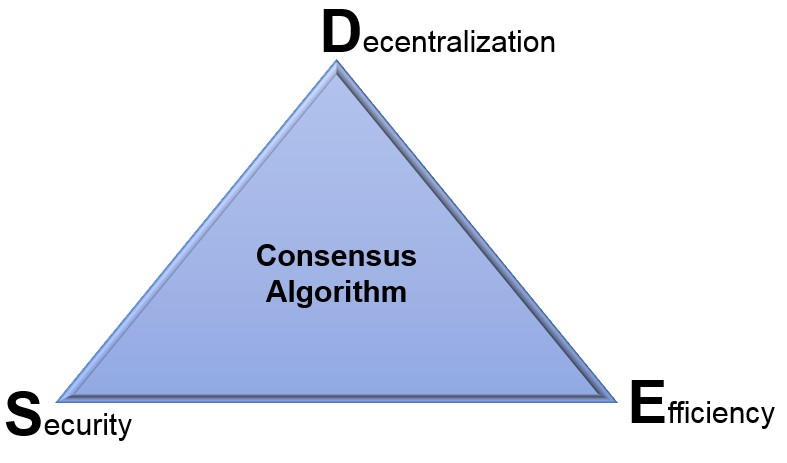
\includegraphics[width=\linewidth]{25}
\caption{Core characteristics}
\label{fig:25}
\end{figure}
According to CAP principle of distributed computing, security, decentralization, and efficiency are impossible to be achieved simultaneously. Trade-off has to be made for the design of consensus mechanism.

HNB team analyzed the current mainstream consensus mechanisms including PoW/PoS/DPoS/PBFT, see Table 6. 

\begin{table*}[hbt]
\caption{Current Mainstream Consensus Mechanisms Analysis}
\centering
\begin{tabular}{p{3cm}p{9cm}p{4cm}}
\toprule
Consensus Mechanism
 & Brief Definition & Concerns \\
\midrule
Proof of Work (PoW): & 
This type of consensus mechanism relies on proof that adequate computational resources have been spent before proposing a value for acceptance by the network. This scheme is used in Bitcoin, Litecoin, and other cryptocurrency Blockchain’s. Currently, it is the only algorithm that has proven to be astonishingly successful against any collusion attacks on a blockchain network
 & 
PoW meets the security and decentralization requirements, but the efficiency is relatively low
\\
\midrule
Proof of Stake (PoS)
 & 
This algorithm works on the idea that a node or user has an adequate stake in the system; that is, the user has invested enough in the system so that any malicious attempt by that user would outweigh the benefits of performing such an attack on the network. This idea was first introduced by Peercoin, and it is going to be used in the Ethereum blockchain version called Serenity. Another important concept in PoS is coin age, which is a criterion derived from the amount of time and number of coins that have not been spent. In this model, the chances of proposing and signing the next block increase with the coin age.
 & 
PoS satisfies decentralization and efficiency, but it lacks security; PoS validates transactions based kind of probability calculation, is vulnerable to attack. 
PoS also fails to avoid nothing-at-the-stake attack
\\
\midrule
Delegated Proof of Stake (DPoS)
 & 
This is an innovation over standard PoS, whereby each node that has a stake in the system can delegate the validation of a transaction to other nodes by voting. It is used in the BitShares blockchain
 & 
DPoS satisfies the efficiency, but not decentralization. The consensus result could be easily controlled/influenced by the nodes of specific interest groups, resulting in the high possibility of the attack by malicious single node.
\\
\midrule
Practical Byzantine Fault Tolerance (PBFT)
 & 
This mechanism achieves state machine replication, which provides tolerance against Byzantine nodes. Various other protocols including PBFT, PAXOS, RAFT, and Federated Byzantine Agreement (FBA) are also being used or have been proposed for use in many different implementations of distributed systems and Blockchain.
 & 
PBFT satisfies decentralization and security, and when the number of nodes increases, the network overhead becomes heavy and it’s difficult to reach consensus efficiently; so not suitable for large network
\\
\bottomrule
\end{tabular}
\label{tab:label}
\end{table*}

The key consideration factors comparison is listed in the table7.

\begin{table*}[hbt]
\caption{Key Consideration Factors Comparison}
\centering
\begin{tabular}{lp{2cm}p{1.5cm}p{1.5cm}p{1.5cm}p{1.5cm}p{1.5cm}p{3cm}r}
\toprule
\qquad
& 
PoW
&
PoS
&
DPoS
&
BFT/PBFT
&
RAFT
&
Dpos + Algorand
\\
\midrule
BFT(Byzantine Fault Tolerance) & 50\%& 50\% &  50\% &  33\%& No &  50\%  \\
\midrule
CFT(Crash Fault Tolerance)  & 50\%& 50\% &  50\% &  33\%& 50\% &  50\%  \\
\midrule
Block Validation Time & BTC: 60 min ETH: 1min & \textless 100 s & \textless 100 s &  \textless 10 s & \textless 5 s &  \textless60 s  \\
\midrule
Scalability & Strong & Strong &  Strong & Weak & Weak &  Strong  \\

\midrule
TPS (Transactions per second) & \textless 100 & \textless 1000 &  \textgreater 500 & \textgreater 1000 & \textgreater 5000 & \textgreater 1000  \\
\midrule
Resource Consumption  & High & Middle &  Low & Low & Low &  Low  \\

\bottomrule
\end{tabular}
\label{tab:label}
\end{table*}


Under current HNB application scenario and economic model, efficiency is the priority so that HNB platform will be able to support the large numbers of concurrent transactions. Massive real-time transactions cannot tolerate long confirmation time. At the same time, the system operating around payments, while the low latency is emphasized, shall not cause double-spending problems, the reliability is crucial. Security is another critical for systems that operate around financial payments and data. As the trades-off, decentralization requirement takes the back seat.

Based on the above analysis and assumptions, HNB architecture embraces an innovative consensus algorithm based on DPoS + Algorand for HNB decentralized economic community blockchain, Figure 25. \\

\begin{figure*}[ht]\centering % Using \begin{figure*} makes the figure take up the entire width of the page
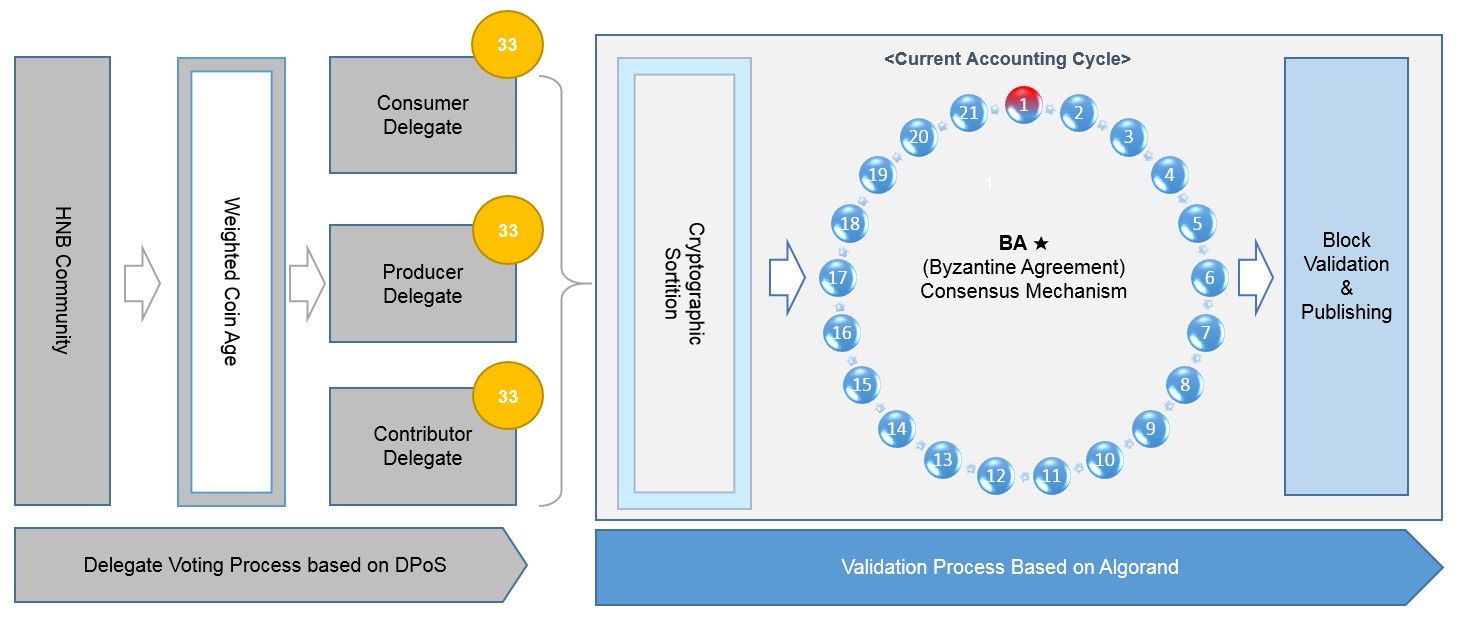
\includegraphics[width=\linewidth]{26}
\caption{HNB decentralized economic community blockchain}
\label{fig:26}
\end{figure*}

\noindent{\textbf {•	Delegate Election Process based on DPoS}}

o	Election of 99 accounting delegates from entire HNB community

o	99 delegates are divided evenly into 3 groups, which represents 3 different interest groups, consumer, producer (or merchant) and contributor. 

o	The constitution of delegates ensures no single interest group can have overwhelming advantage over and impact on the normal operations of the entire community

o	HNB community users vote for candidate based on the weight of their currency and holding time ( Token Age)\\

\noindent{\textbf {•	Validation Process Based on Algorand}}


HNB architecture adopts Algorand as its core consensus algorithm for transaction validation process.

Algorand is a new cryptocurrency that confirms transactions with latency on the order of a minute while scaling to many users. Algorand ensures that users never have divergent views of confirmed transactions, even if some of the users are malicious and the network is temporarily partitioned.

Algorand's design is based on a cryptographic sortition mechanism combined with the BA Byzantine agreement protocol. Algorand avoids targeted attacks at chosen participants using participant replacement at every step. 

For the traditional POW and POS, the essence of mining is to obtain random numbers by computing hash to ensure fairness, and HNA uses the cryptographic sortition in the Algorand algorithm to ensure the fairness and robustness of the transaction validation, while avoiding a large amount of energy-intensive and meaningless calculations to resolve hard cryptographic puzzles.

Summary of HNB approach:

o	Using Algorand algorithm’s \textbf{Cryptographic Sortition} to select 21 accounting nodes including 1 master notes among 99 selected delegates during the current accounting cycle

o	Cryptographic Sortition is an algorithm for choosing a random subset of users according to per-user weights; that is, given a set of weights and the weight of all users. Sortition is implemented using \textbf{Verifiable Random Functions (VRFs)}

o	The selected Master Node proposes a new block. Then we use a new \textbf{Byzantine Agreement (BA)} protocol called \textbf{BA} to reach consensus among 21 accounting nodes

o	\textbf{BA} is designed to guarantee consensus as long as a weighted fraction (a constant greater than 2/3) of the tokens are controlled by honest users

o	The new block is then validated and published to the HNB public blockchain.

So the accounting tasks are performed by the selected accounting nodes to create, verify, sign, and mutual-supervise, which significantly reduces the time and computational costs that are required to create and validate the blocks. 

The selected delegates cannot change the details of the transaction. If the node has behaviors such as trying to do any harm, providing unstable computing power, and computer downtime, the open community or the designated algorithm can quickly block his or her accounting privileges. (Such as offline for long period, no response after election or other behaviors are concluded as abnormal).

\noindent{\textbf {•	Key Considerations of Algorand Algorithm Based Consensus Mechanism}}


o	For traditional POWs and POS, the essence of mining is to obtain accounting rights in a fair manner through proof of work or coin stake. HNB uses the VRF in Algorand's algorithm to guarantee the random selection of accounting nodes, which guarantees the fairness and robustness of accounting while avoiding a large amount of meaningless calculations

o	Algorand mechanism allows users to check whether they are selected to participate in the consensus on the next batch of transactions under secret conditions. Users do not need to keep any private state except for keeping their private keys. After the vote, their identities are exposed. Although they will be corrupted by attackers at this time, the messages they send cannot be revoked. In addition, once the message is generated, the one-time temporary key used for signing is immediately discarded, making it impossible for the attacker to generate any more valid messages

o	Algorand has the feature that participating accounting nodes can be replaced immediately. The attacker may attack the participant when a message is sent during BA process. BA mitigates this attack by requiring all participating accounting nodes to speak just once. Therefore, once a participating accounting node sends a message (and exposes the identity to the attacker), BA will revoke the user's private key and relaunch the sortition process. This avoids a targeted attack after a participant's identity is exposed, such as during DPoS process.

o	HNB consensus mechanism does not include incentives of accounting nodes for specific transaction validation. In HNB economic community, new HGS Token as stable currency will be issued each year with the growth of economic scale, the accounting node will be rewarded for incentives based on the contribution and performance. This will be detailed in the further release HNB economic policies. \\

\noindent{\textbf {•	Summary of HNB Consensus Mechanism Advantages}}

o	DPoS based delegate election takes full account of interests distribution and fairness, and avoid attackers; 

o	Using DPoS to run for delegate nodes will be more stable and relatively high performance than using Algorand to select users with Verifiable Random Functions (VRFs)

o	Fast to reach consensus

o	Algorand’s Cryptographic Sortition ensured that the accounting node is completely random and secretive and specific attacks will not work

o	Scalable to support large number of nodes without performance degrade

o	Ensure Security without heavy computation overhead and energy-saving  

o	Never hard fork

o	High fault-tolerant\\

\subsection{DApp}


HNB Blockchain supports DApp (decentralized application) as one of the core feature of HNB's decentralized economic community.

A DApp has its backend code running on HNB's decentralized peer-to-peer network. In HNB Blockchain, DApp's backend code is realized by Smart Contract. 

Smart contract is the programs run on top of the blockchain and encapsulate the business logic to be executed when certain conditions are met. The frontend could be any JavaScript, along with the web3 library that provides the APIs to communicate with the smart contract in the backend, Figure 26.

\noindent\textbf {DApp = Frontend User Interface + Backend Smart Contract}

HNB DApp includes the following features:

o	Open Source: Source code of app is available to all.

o	Decentralized: Run over HNB Blockchain peer-to-peer network

o	Incentivized: HGS as incentives for node/user which contributing to DApp running

o	Consensus Algorithm: Based on HNB Blockchain’s consensus mechanism\\

\begin{figure}[!hbpt]\centering
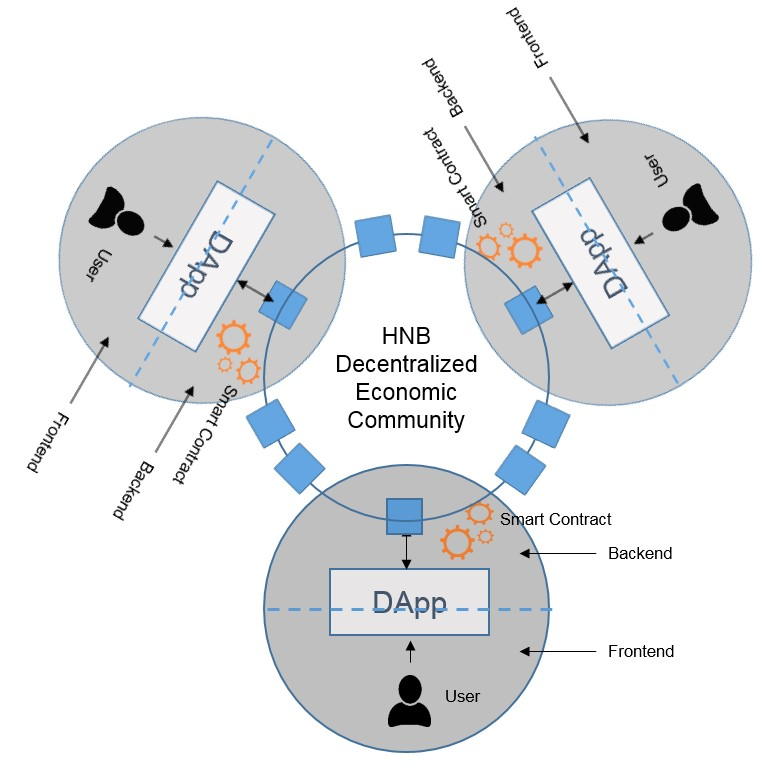
\includegraphics[width=\linewidth]{27}
\caption{DApp}
\label{fig:27}
\end{figure}

\noindent{\textbf {•	DApp Frontend}}

HNB will provide a collection of robust and organic DApps in the community. The Frontend services including but not limited to:

o	Community Governance

o	Auction System

o	Merchant Promotion

o	OTC/C2C Transaction

o	Decentralized CC Exchange

o	Community Events

o	Bulletin Board

o	Asset Management

Some above features described in the user layer and business layer are actually supported by DApps and backend smart contracts embedded with business logic. \\
	
\noindent{\textbf {•	DApp Backend}}

DApp backend services include lightweight or SPV (Simplified Payment Verification) node support, wallet services and payment SDK. 

The purpose of payment SDK is to provide API interface for 3rd party applications, which enables easy integration or redirection of payment process to HNB system, Figure 27.

\begin{figure}[ht]\centering % Using \begin{figure*} makes the figure take up the entire width of the page
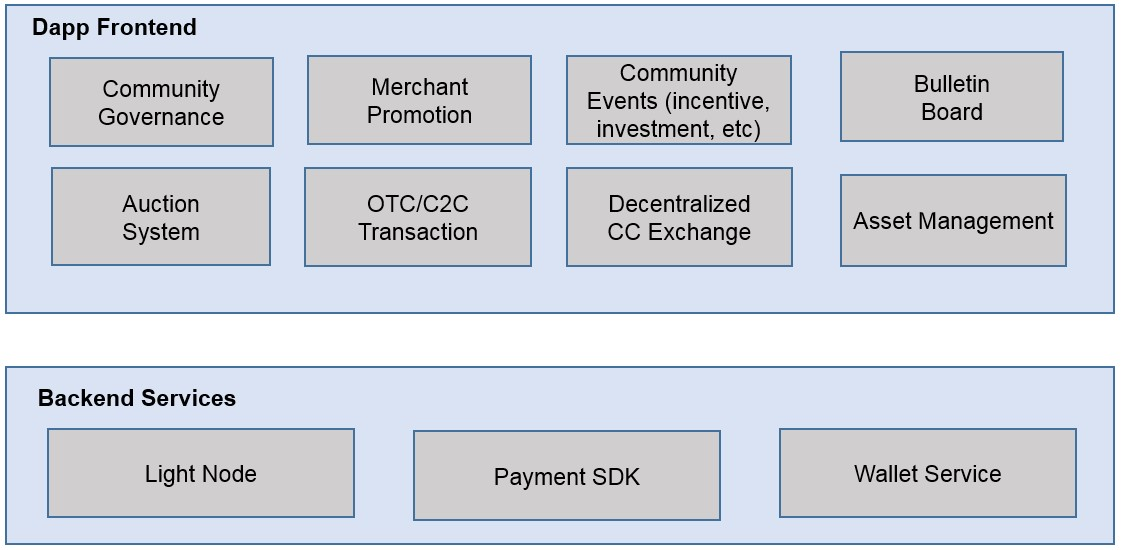
\includegraphics[width=\linewidth]{28}
\caption{DApp Backend}
\label{fig:28}
\end{figure}

\subsection{Security}

HNB team puts security at core of the design of HNB entire architecture.

A series of recent cyber-attacks on digital currencies have drawn attentions to the vulnerabilities of the Blockchain technology. The major security breach incidents like DAO and Bitfinex, robbed $50 m and $150 m respectively by cyber-attacks, raised overwhelming security concerns to the Blockchain technology in the community. Some of the causes identified are due to the newness of programming code behind the technology. 

Despite Blockchain technology is based on robust cybersecurity principles, it is the underlying technology to bolster an ecosystem, applications and the networks, in which the business value is created. It is part of broad business-driven ecosystem as opposed operated in isolation. And where there is an ecosystem, there is vulnerability and weakness exposed to potential attack. 

Blockchain applications can run on platforms and infrastructures in private, public or hybrid environments. The security pyramid made of physical, network, user, application and data, is highly relevant within the context of the operating environments.

HNB security implementation is based on a layered approach as Figure 28 and Table 8:

\begin{figure}[ht]\centering
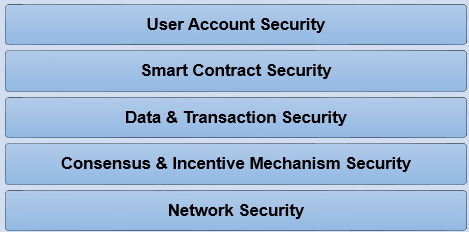
\includegraphics[width=\linewidth]{29}
\caption{HNB blockchain security in layered approach}
\label{fig:29}
\end{figure}

\begin{table*}[hbt]
\caption{HNB Security implementation}
\centering
\begin{tabular}{lp{11cm}p{2cm}r}
\toprule
Layer
 & 
HNB Security implementation\\
\midrule
Network
Security
&
o	TLS (Transport Layer Security) protocol for communication between nodes

o	DDoS (Distributed Denial of Service) detection and prevention

o	Security Hardening for all HNB applications and systems

o	HNB Security Operation Center for monitoring and detection
\\
\midrule
User Account Security
 & 
o	User Registration and Authentication

o	Digital ID Management based on PKI /CA Infrastructure

o	Secured User side client software and data storage encryption

o	Monitoring and freezing abnormal transactions based on algorithm

o	Blacklist mechanism for malicious user accounts
\\
\midrule
Data \& Transaction Security
 & 
o	Digital Signature based on ECDSA for transactions

o	Transaction is digitally signed by user private key and verification based on asymmetric public key to ensure non-repudiation and authenticity

o	Hash SHA algorism for data comparison and validation to ensure integrity and tamperproof

o	Private transaction info encryption for confidentiality of data not required on the chain and visible only for relevant parties
\\
\midrule
Consensus \& Incentive Mechanism Security
&
o	Innovative DPoS+ Algorand Consensus algorithm to prevent single interest group from taking monopolistic attack in the light of interest equilibrium theory

o	Penalty mechanism to increase the risks and costs of malicious attack
\\
\midrule
Smart Contract
 & 
o	User authentication process for smart contract execution

o	Monitoring and freezing abnormal transactions based on algorithm

\\
\midrule
Security
 & 
o	Code audit based on industrial standards and code analysis tools for potential bugs 

o	Penetration test for vulnerabilities detection and fix

\\
\midrule
\bottomrule
\end{tabular}
\label{tab:label}
\end{table*}

The following essential building blocks of security are deployed to protect HNB's Blockchain-based decentralized economic community:

o	Manage the operational policies, risks and compliance.

o	Conduct threat-based risk assessments.

o	Follow privacy-by-design and security-by-design principles.

o	Build a resilient business network.

o	Implement strong access control

o	Deploy robust and secure digital key and certificate management solutions.

o	Assure data security and privacy controls.

o	Address cybersecurity monitoring and incident response.\\




%------------------------------------------------


\section{HNB Project Milestones}


HNB’s core team members are pioneers and early investors in the field of Bitcoin and Blockchain related business activities since 2011. 

The HNB project is officially launched in early 2017 by its core team members. The high level vison and associated project Milestones as Figure 29 and Table 9.

\begin{figure*}[!ht]\centering % Using \begin{figure*} makes the figure take up the entire width of the page
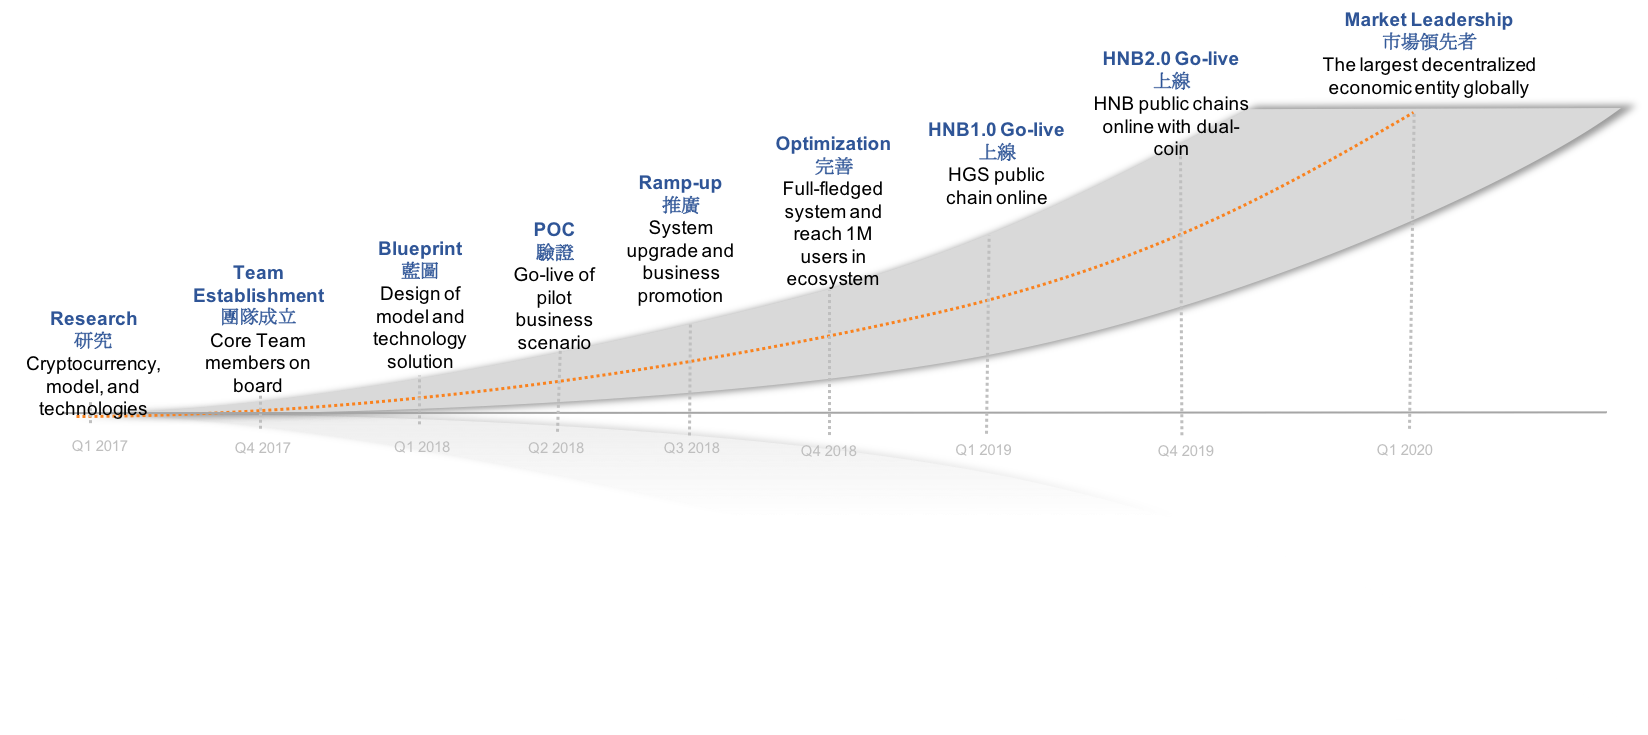
\includegraphics[width=\linewidth]{30}
\caption{HNB Project Milestones}
\label{fig:30}
\end{figure*}

\begin{table*}[!hbt]
\caption{HNB Project Milestones}
\centering
\begin{tabular}{p{2cm}p{3cm}p{11cm}}
\toprule
Timeframe
 & Stage & Key Missions \& Objectives  \\
\midrule
Q1 2017 & 
Research
 & 
Conduct extensive research of cryptocurrency investment, business models and associated technologies\\
\midrule
Q4 2017 & 
Team Establishment 
 & 
Core team members on board\\
\midrule
Q1 2018 & 
Blueprint
 & 
Complete the design of decentralized economic model and underlying technical solutions \& architecture.\\
\midrule
Q2 2018 & 
Proof of Concept
 & 
Go alive of the viable system in the aim to confirm HNB economic mode as its first stage, including merchants store opening, promotion of product to the consumers, etc.
\\
\midrule
Q3 2018 & 
Ramp-up
 & 
Upgrade the system to support larger scale of business scenarios and market promotions\\
\midrule
Q4 2018 & 
Optimization
 & 
Complete the full-fledged HNB system:establishment of entire HNB economic model and smooth operation of various activities. Target to reach 1 million community members in the ecosystem\\
\midrule
Q2 2019 & 
HNB 1.0 go-live
 & 
HGS public chain online\\
\midrule
Q4 2019 & 
HNB 2.0 go-live
 & 
HNB public chain online with Dual-Token mode and full operation of the ecosystem with multiple side chains and inter-chain communication and integration. \\
\midrule
Q1 2020 & 
Market Leadership
 & 
HNB becomes one of the largest decentralized economic entities globally. \\
\bottomrule
\end{tabular}
\label{tab:label}
\end{table*}
%------------------------------------------------

\cleardoublepage

\newpage
\cleardoublepage


\section{HNB Token Structure}

\subsection{Token Issuance}

HNB Foundation proposes to generate and issue 1 Billion ($10^9$) HNB Tokens. The quantities of HNB Token are capped at 1 billion and can be indefinitely split. Further information about when and to whom HNB are proposed to be allocated can be found below.

\subsection{Allocation of HNB Token}
HNB's allocation proportions are shown as Figure 30:

\begin{figure}[ht]\centering
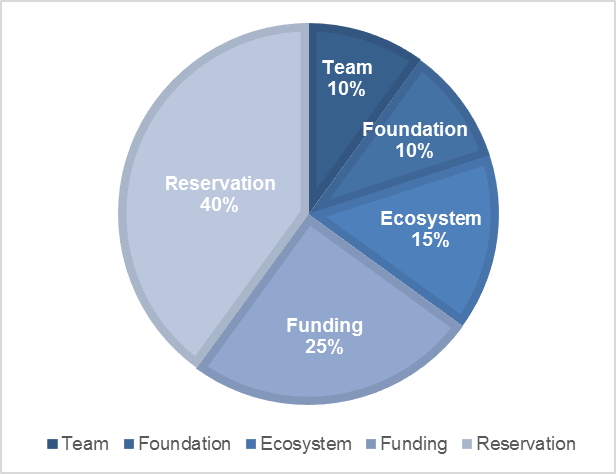
\includegraphics[width=\linewidth]{37}
\caption{HNB's allocation proportions}
\label{fig:37}
\end{figure}

\begin{itemize}
\item{The HNB Token allocation for HNB \textbf{team and partners} will be subject to a long term (2 years) vesting period. The Token release mechanism is 10\% per month after the 14th month of launching. These rules are programmed into a Smart Contract and cannot be changed.}
\item{\textbf{Foundation} is open governance of its resources together with other ecosystem partners, support and advance the technology related to HNB Blockchain networks implementation and are responsible for all matters related to ecosystem membership. Its goal is to transfer the right to the DAO of HNB eventually. There is no locking mechanism for foundation.}
\item{HNBs reserved for the \textbf{Eco-system} are held for end users, to jumpstart the use of HNB platform applications and to encourage participation in the ecosystem such as attracting commercial tenants and their customers from various industries. There is no locking mechanism for Eco-system.}
\item{The portion of \textbf{Funding} is 30\% of total HNB issuances. The fund is raised from Pre-Angel investors, cornerstone investors and private placement. This part builds strong endorsement for the company and enhances great confidence in the market. 50\% of HNB Token held by these group of Investors will be subject to 6 months vesting period. }
\item{\textbf{Reservation portion} is to be held in reserve for further release by the Foundation (in next 40 years). It is an engine for a self-developing community governed by HNB DAO (Decentralized Autonomous Organization). } \\ 

\end{itemize}
\subsection{Fundraising Plan}

The Proceeds raised from HNB Token insurance are in form of ETH.

For further information and updates regarding the Fundraising and Proceeds raised, prospective participants are invited to send a request.\\

%------------------------------------------------

\section{HNB Core Team and Advisors}

\subsection{Core Team (Figure 31 and Table 10)}
The team has been established with 14 members, but no more than 22. 

Team members are from Operations Department, Development of Model Design and System Development and Market Research and Support Department, respectively. All members have at least a Master’s degree, or are graduates from well-known colleges and universities such as Purdue University, Fudan University, Jiaotong University and Tongji University. Moreover, they've been working in the research institute of School of Economics, large investment institutions as CSO and famous companies such as Alipay, HP and PWC, etc.\\

\begin{figure*}[!hbt]\centering % Using \begin{figure*} makes the figure take up the entire width of the page
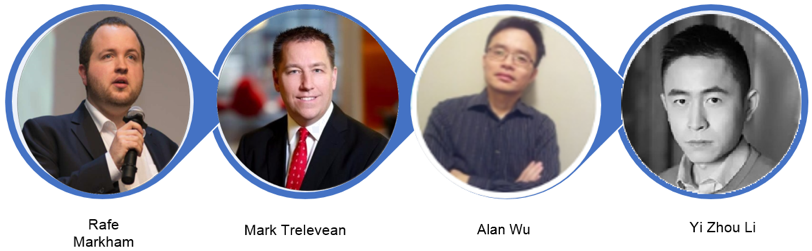
\includegraphics[width=\linewidth]{32}
\caption{Core Team}
\label{fig:32}
\end{figure*}

\begin{table*}[!hbt]
\caption{Core Team}
\centering
\begin{tabular}{lp{13cm}p{2cm}r}
\toprule
Name
 & 
Brief Introduction\\
\midrule
Rafe Markham
 & 
Researcher of global economy and culture. Specializing in econometrics, macro-economy, quantitative Methods. Familiar with the economies of Europe, USA, Russia and China. Involved in cryptocurrency investment and Blockchain research for many years, deeply understand the insight of DAO. 

\textbf{Economy
Master of University of Nottingham}
\\
\midrule
Mark Trelevean
 & 
Specializing in Strategic planning, change management, and new business building, Mark brings expert evaluation, deep experience and innovation to bridging systems, processes and people solutions. Involved projects include IOT Data Collection and Analytics, Cloud Back Office for SMB, Systems Review for a large NGO, and the latest Fintech, including Blockchain and Digital Ledger envisioning. 

\textbf{Computer Science 
Bachelor of York University }
\\
\midrule
Yi Zhou Li
 & 
Expert in product design, user experience design and service design research, and maketing for mobile internet and new media.
Entrepreneur in the area of AI, Consumer Electronics and blockchain
 

\textbf{Design Science
Doctor of Tsinghua university}
\\
\midrule
Alan Wu
 & 
As Leader of Enterprise Architect for HPE / DXC Canada many years, Alan has a breadth of management experience to lead a team to deliver complex IT services and drive IT transformation for better business outcomes. Alan is a blockchain technology advocator. He has in-depth experience in HP Cloud Service Automation, vCloud Automation Center and Openstack solution and implementation. 

\textbf{Computer Science
Bachelor of Fudan University}
\\
\bottomrule
\end{tabular}
\label{tab:label}
\end{table*}

\subsection{Investors and Advisors (Figure 32)}

\begin{figure*}[!hbt]\centering % Using \begin{figure*} makes the figure take up the entire width of the page
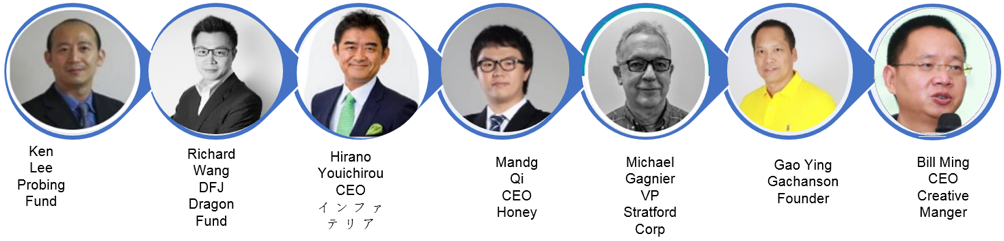
\includegraphics[width=\linewidth]{33}
\caption{Investors and Advisors}
\label{fig:33}
\end{figure*}

\subsection{Institutional Investors (Figure 33)}

\begin{figure*}[!ht]\centering % Using \begin{figure*} makes the figure take up the entire width of the page
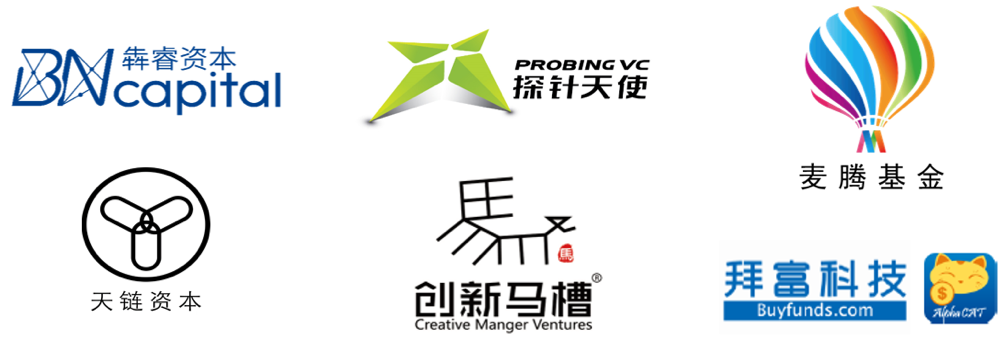
\includegraphics[width=\linewidth]{34}
\caption{Institutional Investors}
\label{fig:36}
\end{figure*}

\subsection{Business Partners (Figure 34)}

\begin{figure*}[!ht]\centering % Using \begin{figure*} makes the figure take up the entire width of the page

\includegraphics[width=\linewidth]{35}
\caption{Business Partners}
\label{fig:35}
\end{figure*}

\cleardoublepage
%------------------------------------------------
\newpage
\cleardoublepage

\section{Risk Disclosure and Disclaimer}

\subsection{Risk Disclosure and Approval}

Systematic risk refers to the possible changes in earnings due to the overall common factors that affect the returns on all securities in the same way. For example, the policy risk - at present, government's regulatory policies for the Blockchain projects and the financing of the listing methods are not yet clear, and there is a certain possibility of economic loss of participants due to policy reasons; among the market risk, if the overall value of the digital asset market is over estimated, then the investment risk will be increased, participants may expect relative high growth of listed project, but these high expectations may not be realized. At the same time, systemic risks include a series of force majeure factors including, but not limited to, natural disasters, widespread worldwide breakdown of computer networks, political instability, etc.

\noindent{\textbf{Lack of Supervision Risk}}\\
Digital asset transactions, including HNC, are highly uncertain. As currently there is no strong supervision in the field of digital asset transactions, there is a risk that electronic digital currencies will skyrocket or collapse and is subject to the risk of market manipulation by bankers, as a result, it may be difficult for individual participants lack of experience to withstand the asset shock and psychological stress caused by market instability. Although academics, the government media, etc. will occasionally give suggestions for cautious participation, there still are no written supervisory methods and provisions, therefore, currently such risks are hard to be effectively circumvented.

\noindent{\textbf {Risk of Promulgated Regulation}}\\
It is undeniable that in the foreseeable future, the regulatory rules will be promulgated to constrain the blockchain and electronic digital currency areas. If regulation entities conduct the standardization management for this sector, the digital currencies purchased during the listing period may be affected, including but not limited to the fluctuations or restrictions in price and marketability.

\noindent{\textbf {Inter-team Risk}}\\
Currently there are numerous teams and projects in the Blockchain technology area, the competition is very fierce, and there is a strong market competition and project operating pressure. The realization of breakthrough and wide recognition of HNB project from many outstanding projects depends on its own team capabilities, vision planning and other aspects, but it is also affected by many competitors in the market and even the oligarchy, during which there is the possibility of facing vicious competition.

\noindent{\textbf {Risk of Team Itself}}\\
HNB brings together a team of people who are both dynamic and strong, attracting the experienced practitioners and experienced technology developers in the area of Blockchain. As a leader in the industry, the stability and cohesion within the team are crucial to the overall development of HNB. In the future development, the core personnel may leave or the conflict may happen within the team, which may adversely impact HNB team.

\noindent{\textbf {Risk of Project co-ordination and Marketing}}\\
HNB’s founding team will spare no efforts to achieve the development goals set out in the white paper and extend the growth space of project. Currently HNB has established a relatively mature business model analysis; however, the presence of unforeseen factors in the overall industry trends, existing business model and overall idea may not properly meet market demands, leading to unpredictable consequences in earning. Meanwhile, as this white paper may be adjusted with the detail updating of the project, if the updated details of the project are not timely obtained by market participants, or the public do not understand the latest progress of the project, participants or the public may lack of awareness of the project because of information asymmetry, all those factors will affect the subsequent development of the project.

\noindent{\textbf {Project's Technical Risk}}\\
This project is built based on the cryptography algorithm, the rapid development of cryptography is bound to bring the potential risk of decryption; at the same time, block chain, distributed ledger, decentralization and tamper-resistance and other technologies support the core business development, HNB team can’t fully guarantee the implementation of technologies; during the process of project update and adjustment, some loopholes can be remedied by issuing patches, but the degree of impact caused by the loopholes can’t be guaranteed.

\noindent{\textbf {Risk of Hacking and Crime}}\\
In terms of security, the amount of individual supporter is small, but the total number is large, which also places high demands on the safety and security of the project. Electronic digital currency has anonymity, difficult to traceability and other characteristics, using digital money to transfer the funds obtained from criminal offenses is also a criminal act and will be punished by law.

\noindent{\textbf {Other Unknown Risks at Present }}\\
With the continuous development of Blockchain technology and industry's overall situation, HNB may face some unforeseen risks. Before participating in the decision-makings, participants should fully understand team's background, the overall framework and concepts of the project; reasonably adjust your vision and rationally participate in digital currency crowdfunding.

\subsection{Disclaimer}

HNB is a public welfare, non-profit system, the internal reward mechanism, operation and maintenance mechanisms adopted by the system in the future are based on virtual digital assets (ie, virtual goods), rather than monetary incentives. The digital currency generated by system can be used as reward for system maintenance, but in order to meet the requirements of resources exchange among system, other system or other social subjects, it requires the intervention of a certain amount of ETH and other virtual digital assets. Accordingly, the assets acquired through the marketing of HNB are only similar virtual digital assets such as BTC, ETH, NEO and other tokens.

HNC is a kind of digital currency used by HNB for its usage scenarios; it is a virtualization rewards mechanism for operating the system, not a monetary return. Therefore, the exchange of HNC is not an investment. Holding HNC does not represent the ownership of HNB or HNB applications, HNB does not grant any individual any rights to participate, control, or make any decision about HNB and HNB applications. HNC holders can participate in HNB platform's usage scenarios, but can’t be directly convert HNC into currency. The value goal of creation of HNC is to create the application value of HNB application platform and usage scenarios and scarcity experience of the virtual goods for the participants and holders rather than the monetary value or the transaction value. We can’t guarantee that HNC will add value, and it is also possible that under certain circumstances there will be a decline in its psychological cognition value. Given the unpredictable circumstances, the goals outlined in this white paper may change. Although the team will try its best to achieve all of the objectives in this white paper, all individuals and groups that purchase HNC will at their own risks.

This white paper is for informational purposes only and does not constitute any investment advice, investment intention or solicitation of investment. This White Paper does not constitute or can't be understood as any sale or purchase, any offer to buy or sell, any type of securities or any form of contract or guarantee.

The participants of HNB project marketing must read HNB White Paper, fully understand the technical features HNB and marketing risk-return characteristics of HNB, fully consider your own risk tolerance and make rational judgment and prudent decision, participation in the project means understanding and acceptance of project risk, and is willing to bear all the corresponding results or consequences for such decision.

%------------------------------------------------
%\phantomsection
%\section*{Acknowledgments} % The \section*{} command stops section numbering

%\addcontentsline{toc}{section}{Acknowledgments} % Adds this section to the table of contents
%So long and thanks for all the xxx 

%----------------------------------------------------------------------------------------
%	REFERENCE LIST
%----------------------------------------------------------------------------------------

\section{References}

\noindent{[1] Satoshi Nakamoto. Bitcoin: A Peer-to-Peer Electronic Cash System. https://bitcoin.org/ bitcoin.pdf. Oct 2008\\}


\noindent{[2] Vitalik Buterin:Ethereum White Paper: A Next-Generation Smart Contract and Decentralized Application Platform. \\https://github.com/ethereum/wiki/wiki/White-Paper. \\}


\noindent{[3] Hyperledger: Hyperledger Arch WG Paper 1 Consensus, https://www.hyperledger.org/resources/publications\#white-papers \\}


\noindent{[4] Hyperledger: Hyperledger Arch WG Paper 2 SmartContracts https://www.hyperledger.org/resources/publications\#white-papers \\}


\noindent{[5] EOS.IO Technical White Paper v2, https://github.com\\/EOSIO/Documentation/blob/master/TechnicalWhitePaper.md \\}


\noindent{[6] Chine Blockchain Development Forum  Blockchain—Reference Architecture May 2017 http://www.cbdforum.cn/bcweb/index/bz/1-0.html \\}


\noindent{[7] Chris Dannen: Introducing Ethereum and Solidity 2017 \\}


\noindent{[8] Imran Bashir Mastering Blockchain 2017 Packt Publishing \\}


\noindent{[9] Algorand: Scaling Byzantine Agreements for Cryptocurrencies ,https://www.algorand.com/whitepapers/ \\}


%----------------------------------------------------------------------------------------

\end{document}